\documentclass[10pt,fleqn]{article} % Default font size and left-justified equations
\usepackage[%
    pdftitle={Modélisation dynamique},
    pdfauthor={Xavier Pessoles}]{hyperref}

    
%%%%%%%%%%%%%%%%%%%%%%%%%%%%%%%%%%%%%%%%%
% Original author:
% Mathias Legrand (legrand.mathias@gmail.com) with modifications by:
% Vel (vel@latextemplates.com)
% License:
% CC BY-NC-SA 3.0 (http://creativecommons.org/licenses/by-nc-sa/3.0/)
%%%%%%%%%%%%%%%%%%%%%%%%%%%%%%%%%%%%%%%%%

%----------------------------------------------------------------------------------------
%	VARIOUS REQUIRED PACKAGES AND CONFIGURATIONS
%----------------------------------------------------------------------------------------

%\usepackage[top=2.5cm,bottom=2cm,left=2cm,right=2cm,headsep=40pt,a4paper]{geometry} % Page margins
\usepackage[top=2cm,bottom=2cm,left=2cm,right=2cm,a4paper]{geometry} % Page margins

\usepackage{graphicx} % Required for including pictures

\usepackage{lipsum} % Inserts dummy text

\usepackage{tikz} % Required for drawing custom shapes

\usepackage[francais]{babel} % English language/hyphenation
\frenchbsetup{StandardLists=true} % Pour éviter la collision babel enumitem pour les listes

\usepackage{enumitem} % Customize lists
\setlist{nolistsep} % Reduce spacing between bullet points and numbered lists

\usepackage{booktabs} % Required for nicer horizontal rules in tables

\usepackage{xcolor} % Required for specifying colors by name
%\definecolor{ocre}{RGB}{243,102,25} % Define the orange color used for highlighting throughout the book
 \definecolor{ocre}{RGB}{49,133,156} % Couleur ''bleue''
\definecolor{violetf}{RGB}{112,48,160} % Couleur ''violet''
\usepackage{enumitem}
\usepackage{pifont} % Pour les dinglist
\usepackage{multicol}
\usepackage{array} % Centrage vertical dans les tableaux
\usepackage{schemabloc}

%----------------------------------------------------------------------------------------
%	FONTS
%----------------------------------------------------------------------------------------
\usepackage{bm}
\usepackage{multicol}
\usepackage{siunitx}
\sisetup{output-decimal-marker = {,}}


\usepackage{avant} % Use the Avantgarde font for headings
%\usepackage{times} % Use the Times font for headings
%\usepackage{mathptmx} % Use the Adobe Times Roman as the default text font together with math symbols from the Sym­bol, Chancery and Com­puter Modern fonts
\usepackage[adobe-utopia]{mathdesign}
\usepackage{microtype} % Slightly tweak font spacing for aesthetics
\usepackage[utf8]{inputenc} % Required for including letters with accents
\usepackage[T1]{fontenc} % Use 8-bit encoding that has 256 glyphs

%----------------------------------------------------------------------------------------
%	BIBLIOGRAPHY AND INDEX
%----------------------------------------------------------------------------------------

%\usepackage[style=alphabetic,citestyle=numeric,sorting=nyt,sortcites=true,autopunct=true,babel=hyphen,hyperref=true,abbreviate=false,backref=true,backend=biber]{biblatex}
\usepackage[style=alphabetic,citestyle=numeric,sorting=nyt,sortcites=true,autopunct=true,hyperref=true,abbreviate=false,backref=true,backend=biber]{biblatex}
\addbibresource{bibliography.bib} % BibTeX bibliography file
\defbibheading{bibempty}{}

\usepackage{calc} % For simpler calculation - used for spacing the index letter headings correctly
\usepackage{makeidx} % Required to make an index
\makeindex % Tells LaTeX to create the files required for indexing

%----------------------------------------------------------------------------------------
%	MAIN TABLE OF CONTENTS
%----------------------------------------------------------------------------------------

\usepackage{titletoc} % Required for manipulating the table of contents

\setcounter{tocdepth}{2}     % Dans la table des matieres
\setcounter{secnumdepth}{2}

\contentsmargin{0cm} % Removes the default margin

% Part text styling
\titlecontents{part}[0cm]
{\addvspace{20pt}\centering\large\bfseries}
{}
{}
{}

% Chapter text styling
\titlecontents{chapter}[1.25cm] % Indentation
{\addvspace{12pt}\large\sffamily\bfseries} % Spacing and font options for chapters
{\color{ocre!60}\contentslabel[\Large\thecontentslabel]{1.25cm}\color{ocre}} % Chapter number
{\color{ocre}}  
{\color{ocre!60}\normalsize\;\titlerule*[.5pc]{.}\;\thecontentspage} % Page number

% Section text styling
\titlecontents{section}[1.25cm] % Indentation
{\addvspace{3pt}\sffamily\bfseries} % Spacing and font options for sections
{\color{ocre!60}\contentslabel[\thecontentslabel]{1.25cm} \color{ocre}} % Section number
{\color{ocre}}
{\hfill\color{ocre!60}\thecontentspage} % Page number
[]

% Subsection text styling
\titlecontents{subsection}[1.25cm] % Indentation
{\addvspace{1pt}\sffamily\small} % Spacing and font options for subsections
{\contentslabel[\thecontentslabel]{1.25cm}} % Subsection number
{}
{\ \titlerule*[.5pc]{.}\;\thecontentspage} % Page number
[]


% Subsection text styling
\titlecontents{subsubsection}[1.25cm] % Indentation
{\addvspace{1pt}\sffamily\small} % Spacing and font options for subsections
{\contentslabel[\thecontentslabel]{1.25cm}} % Subsection number
{}
{\ \titlerule*[.5pc]{.}\;\thecontentspage} % Page number
[]

% List of figures
\titlecontents{figure}[0em]
{\addvspace{-5pt}\sffamily}
{\thecontentslabel\hspace*{1em}}
{}
{\ \titlerule*[.5pc]{.}\;\thecontentspage}
[]

% List of tables
\titlecontents{table}[0em]
{\addvspace{-5pt}\sffamily}
{\thecontentslabel\hspace*{1em}}
{}
{\ \titlerule*[.5pc]{.}\;\thecontentspage}
[]

%----------------------------------------------------------------------------------------
%	MINI TABLE OF CONTENTS IN PART HEADS
%----------------------------------------------------------------------------------------

% Chapter text styling
\titlecontents{lchapter}[0em] % Indenting
{\addvspace{15pt}\large\sffamily\bfseries} % Spacing and font options for chapters
{\color{ocre}\contentslabel[\Large\thecontentslabel]{1.25cm}\color{ocre}} % Chapter number
{}  
{\color{ocre}\normalsize\sffamily\bfseries\;\titlerule*[.5pc]{.}\;\thecontentspage} % Page number

% Section text styling
\titlecontents{lsection}[0em] % Indenting
{\sffamily\small} % Spacing and font options for sections
{\contentslabel[\thecontentslabel]{1.25cm}} % Section number
{}
{}

% Subsection text styling
\titlecontents{lsubsection}[.5em] % Indentation
{\normalfont\footnotesize\sffamily} % Font settings
{}
{}
{}

%----------------------------------------------------------------------------------------
%	PAGE HEADERS
%----------------------------------------------------------------------------------------

\usepackage{fancyhdr} % Required for header and footer configuration



\pagestyle{fancy}
 \renewcommand{\headrulewidth}{0pt}
 \fancyhead{}
 
 % ENTETES de page
 \fancyhead[L]{%
 \begin{tikzpicture}[overlay]
\node(logo) at (1,0)
    {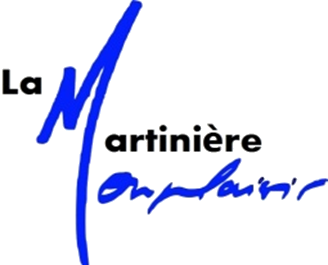
\includegraphics[width=2cm]{logo_lycee.png}};
\end{tikzpicture}
 %\noindent\begin{minipage}[c]{2.6cm}%
 %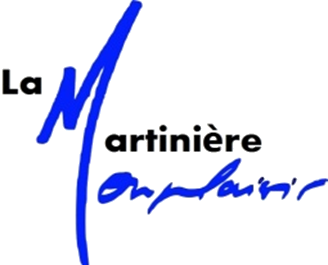
\includegraphics[width=2cm]{logo_lycee.png}%
 %\end{minipage}
}

\fancyhead[C]{\rule{8cm}{.5pt}}

 \fancyhead[R]{%
 \noindent\begin{minipage}[c]{3cm}
 \begin{flushright}
 \footnotesize{\textit{\textsf{\xxtete}}}%
 \end{flushright}
 \end{minipage}
}

 \fancyfoot{}
 % PIEDS de page
\fancyfoot[C]{\rule{12cm}{.5pt}}
\renewcommand{\footrulewidth}{0.2pt}
\fancyfoot[C]{\footnotesize{\bfseries \thepage}}
\fancyfoot[L]{ 
\begin{minipage}[c]{.4\linewidth}
\noindent\footnotesize{{\xxauteur}}
\end{minipage}}

\fancyfoot[R]{\footnotesize{\xxpied}
\ifthenelse{\isodd{\value{page}}}{
\begin{tikzpicture}[overlay]
\node[shape=rectangle, 
      rounded corners = .25 cm,
	  draw= ocre,
	  line width=2pt, 
	  fill = ocre!10,
	  minimum width  = 2.5cm,
	  minimum height = 3cm,] at (\xxposongletx,\xxposonglety) {};
\node at (\xxposonglettext,\xxposonglety) {\rotatebox{90}{\textbf{\large\color{ocre}{\xxonglet}}}};
%{};
\end{tikzpicture}}{}
}



%
%
%
% Removes the header from odd empty pages at the end of chapters
\makeatletter
%\renewcommand{\cleardoublepage}{
%\clearpage\ifodd\c@page\else
%\hbox{}
%\vspace*{\fill}
%\thispagestyle{empty}
%\newpage
%\fi}

%\fancypagestyle{plain}{%
%\fancyhf{} % vide l’en-tête et le pied~de~page.
%%\fancyfoot[C]{\bfseries \thepage} % numéro de la page en cours en gras
%% et centré en pied~de~page.
%\fancyfoot[R]{\footnotesize{\xxpied}}
%\fancyfoot[C]{\rule{12cm}{.5pt}}
%\renewcommand{\footrulewidth}{0.2pt}
%\fancyfoot[C]{\footnotesize{\bfseries \thepage}}
%\fancyfoot[L]{ 
%\begin{minipage}[c]{.4\linewidth}
%\noindent\footnotesize{{\xxauteur}}
%\end{minipage}}}

\fancypagestyle{plain}{%
\fancyhf{} % vide l’en-tête et le pied~de~page.
\fancyfoot[C]{\rule{12cm}{.5pt}}
\renewcommand{\footrulewidth}{0.2pt}
\fancyfoot[C]{\footnotesize{\bfseries \thepage}}
\fancyfoot[L]{ 
\begin{minipage}[c]{.4\linewidth}
\noindent\footnotesize{{\xxauteur}}
\end{minipage}}
\fancyfoot[R]{\footnotesize{\xxpied}}
}




%----------------------------------------------------------------------------------------
%	THEOREM STYLES
%----------------------------------------------------------------------------------------

% Conflit avec la police adobe
%\usepackage{amsmath,amsfonts,amssymb,amsthm} % For math equations, theorems, symbols, etc
\usepackage{amsmath,amsthm}

\newcommand{\intoo}[2]{\mathopen{]}#1\,;#2\mathclose{[}}
\newcommand{\ud}{\mathop{\mathrm{{}d}}\mathopen{}}
\newcommand{\intff}[2]{\mathopen{[}#1\,;#2\mathclose{]}}
%\newtheorem{notation}{Notation}[chapter]
\newtheorem{notation}{Notation}[section]

% Boxed/framed environments
\newtheoremstyle{ocrenumbox}% % Theorem style name
{0pt}% Space above
{0pt}% Space below
{\normalfont}% % Body font
{}% Indent amount
{\small\bf\sffamily\color{ocre}}% % Theorem head font
{\;}% Punctuation after theorem head
{0.25em}% Space after theorem head
{\small\sffamily\color{ocre}\thmname{#1}\nobreakspace\thmnumber%{\@ifnotempty{#1}{}\@upn{#2}}% Theorem text (e.g. Theorem 2.1)
\thmnote{\nobreakspace\the\thm@notefont\sffamily\bfseries\color{black}---\nobreakspace#3.}} % Optional theorem note
\renewcommand{\qedsymbol}{$\blacksquare$}% Optional qed square


% Boite pour les corriges
\newtheoremstyle{correctionbox}% % Theorem style name
{0pt}% Space above
{0pt}% Space below
{\normalfont}% % Body font
{}% Indent amount
{\small\bf\sffamily\color{violet}}% % Theorem head font
{\;}% Punctuation after theorem head
{0.25em}% Space after theorem head
{\small\sffamily\color{ocre}\thmname{#1}\nobreakspace\thmnumber%{\@ifnotempty{#1}{}\@upn{#2}}% Theorem text (e.g. Theorem 2.1)
\thmnote{\nobreakspace\the\thm@notefont\sffamily\bfseries\color{black}---\nobreakspace#3.}} % Optional theorem note
\renewcommand{\qedsymbol}{$\blacksquare$}% Optional qed square



\newtheoremstyle{blacknumex}% Theorem style name
{5pt}% Space above
{5pt}% Space below
{\normalfont}% Body font
{} % Indent amount
{\small\bf\sffamily}% Theorem head font
{\;}% Punctuation after theorem head
{0.25em}% Space after theorem head
{\small\sffamily{\tiny\ensuremath{\blacksquare}}\nobreakspace\thmname{#1}\nobreakspace\thmnumber%{\@ifnotempty{#1}{}\@upn{#2}}% Theorem text (e.g. Theorem 2.1)
\thmnote{\nobreakspace\the\thm@notefont\sffamily\bfseries---\nobreakspace#3.}}% Optional theorem note

\newtheoremstyle{blacknumbox} % Theorem style name
{0pt}% Space above
{0pt}% Space below
{\normalfont}% Body font
{}% Indent amount
{\small\bf\sffamily}% Theorem head font
{\;}% Punctuation after theorem head
{0.25em}% Space after theorem head
{\small\sffamily\thmname{#1}\nobreakspace 
\thmnote{\nobreakspace\the\thm@notefont\sffamily\bfseries---\nobreakspace#3.}}% Optional theorem note

% Non-boxed/non-framed environments
\newtheoremstyle{ocrenum}% % Theorem style name
{5pt}% Space above
{5pt}% Space below
{\normalfont}% % Body font
{}% Indent amount
{\small\bf\sffamily\color{ocre}}% % Theorem head font
{\;}% Punctuation after theorem head
{0.25em}% Space after theorem head
{\small\sffamily\color{ocre}\thmname{#1}\nobreakspace%\thmnumber{\@ifnotempty{#1}{}\@upn{#2}}% Theorem text (e.g. Theorem 2.1)
\thmnote{\nobreakspace\the\thm@notefont\sffamily\bfseries\color{black}---\nobreakspace#3.}} % Optional theorem note
\renewcommand{\qedsymbol}{$\blacksquare$}% Optional qed square
\makeatother

% Environnement pour les titres de parties
\newtheoremstyle{partiebox} 
{0pt}% Space above
{0pt}% Space below
{\normalfont}% Body font
{}% Indent amount
{\small\bf\sffamily}% Theorem head font
{\;}% Punctuation after theorem head
{0.25em}% Space after theorem head




% Defines the theorem text style for each type of theorem to one of the three styles above
\newcounter{dummy} 
\numberwithin{dummy}{section}
\theoremstyle{ocrenumbox}
%\newtheorem{theoremeT}[dummy]{Théorème}
\newtheorem{theoremeT}[dummy]{Théorème}
\newtheorem{resultatT}[dummy]{Résultat}
\newtheorem{savoirT}[dummy]{Savoir}
\newtheorem{methodeT}[dummy]{Méthode}
\newtheorem{objectifT}[dummy]{Objectif}
%\newtheorem{problem}{Problem}[chapter]
\newtheorem{problem}{Problem}[section]
%\newtheorem{exerciseT}{Exercise}[chapter]
\newtheorem{exerciseT}{Exercice}[section]

\theoremstyle{blacknumex}
%\newtheorem{exampleT}{Example}[chapter]
\newtheorem{exempleT}{Exemple}[section]
\newtheorem{termT}{Terminal\\}[section]
\newtheorem{pyT}{Python\\}[section]
\newtheorem{sciT}{Scilab\\}[section]
\newtheorem{pseudoT}{Pseudo Code\\}[section]
\newtheorem{sqlT}{SQL\\}[section]

\theoremstyle{blacknumbox}
%\newtheorem{vocabulary}{Vocabulary}[chapter]
\newtheorem{vocabulary}{Vocabulaire}[section]
%\newtheorem{definitionT}{Definition}[section]
\newtheorem{definitionT}{Définition}[section]
\newtheorem{propT}{Propriété}[section]
\newtheorem{rappelT}{Rappel}[section]
\newtheorem{demoT}{Démonstration}[section]
\newtheorem{corollaryT}[dummy]{Corollaire}
\newtheorem{hypoT}{Hypothèse(s)}

\theoremstyle{ocrenum}
\newtheorem{proposition}[dummy]{Proposition}

\theoremstyle{partiebox}
\newtheorem{titrepartieT}[]{}
\newtheorem{titrechapitreT}[]{}

\theoremstyle{correctionbox}
\newtheorem{correctionT}[dummy]{\color{violet}{Correction}}

%----------------------------------------------------------------------------------------
%	DEFINITION OF COLORED BOXES
%----------------------------------------------------------------------------------------

\RequirePackage[framemethod=tikz]{mdframed} % Required for creating the theorem, definition, exercise and corollary boxes

% Theorem box
\newmdenv[skipabove=7pt,
skipbelow=7pt,
backgroundcolor=ocre!10,
linecolor=ocre,
innerleftmargin=5pt,
innerrightmargin=5pt,
innertopmargin=5pt,
leftmargin=0cm,
rightmargin=0cm,
innerbottommargin=5pt]{tBox}


% Correction
\newmdenv[skipabove=7pt,
skipbelow=7pt,
backgroundcolor=violet!10,
linecolor=violet,
innerleftmargin=5pt,
innerrightmargin=5pt,
innertopmargin=5pt,
leftmargin=0cm,
rightmargin=0cm,
innerbottommargin=5pt]{coBox}


% Exercise box	  
\newmdenv[skipabove=7pt,
skipbelow=7pt,
rightline=false,
leftline=true,
topline=false,
bottomline=false,
backgroundcolor=ocre!10,
linecolor=ocre,
innerleftmargin=5pt,
innerrightmargin=5pt,
innertopmargin=5pt,
innerbottommargin=5pt,
leftmargin=0cm,
rightmargin=0cm,
linewidth=4pt]{eBox}	

% Definition box
\newmdenv[skipabove=7pt,
skipbelow=7pt,
rightline=false,
leftline=true,
topline=false,
bottomline=false,
backgroundcolor=ocre!10,
linecolor=ocre,
innerleftmargin=5pt,
innerrightmargin=5pt,
innertopmargin=0pt,
leftmargin=0cm,
rightmargin=0cm,
linewidth=4pt,
innerbottommargin=0pt]{dBox}	

% Demonstration box
\newmdenv[skipabove=7pt,
skipbelow=7pt,
rightline=false,
leftline=true,
topline=false,
bottomline=false,
%backgroundcolor=ocre!10,
linecolor=ocre,
innerleftmargin=5pt,
innerrightmargin=5pt,
innertopmargin=0pt,
leftmargin=0cm,
rightmargin=0cm,
linewidth=4pt,
innerbottommargin=0pt]{demoBox}	

% Corollary box
\newmdenv[skipabove=7pt,
skipbelow=7pt,
rightline=false,
leftline=true,
topline=false,
bottomline=false,
linecolor=gray,
backgroundcolor=black!5,
innerleftmargin=5pt,
innerrightmargin=5pt,
innertopmargin=5pt,
leftmargin=0cm,
rightmargin=0cm,
linewidth=4pt,
innerbottommargin=5pt]{cBox}


% Hypothèses
\newmdenv[skipabove=7pt,
skipbelow=7pt,
rightline=false,
leftline=true,
topline=false,
bottomline=false,
linecolor=gray,
backgroundcolor=black!5,
innerleftmargin=5pt,
innerrightmargin=5pt,
innertopmargin=5pt,
leftmargin=0cm,
rightmargin=0cm,
linewidth=4pt,
innerbottommargin=5pt]{hyBox}


% Boite pour le titre de la partie (pBox)
\newmdenv[skipabove=7pt,
skipbelow=7pt,
rightline=true,
leftline=false,
topline=false,
bottomline=false,
linecolor=ocre,
backgroundcolor=none,
innerleftmargin=5pt,
innerrightmargin=5pt,
innertopmargin=5pt,
leftmargin=0cm,
rightmargin=0cm,
linewidth=4pt,
innerbottommargin=5pt]{pBox}

% Boite pour le titre du chapitre (chBox)
\newmdenv[skipabove=7pt,
skipbelow=7pt,
rightline=false,
leftline=true,
topline=false,
bottomline=false,
linecolor=ocre,
%backgroundcolor=black!5,
innerleftmargin=5pt,
innerrightmargin=5pt,
innertopmargin=5pt,
leftmargin=0cm,
rightmargin=0cm,
linewidth=4pt,
innerbottommargin=5pt]{chBox}


% Boite pour les exemples
\newmdenv[skipabove=7pt,
skipbelow=7pt,
rightline=false,
leftline=true,
topline=false,
bottomline=false,
linecolor=gray,
backgroundcolor=white,
innerleftmargin=5pt,
innerrightmargin=5pt,
innertopmargin=5pt,
leftmargin=0cm,
rightmargin=0cm,
linewidth=4pt,
innerbottommargin=5pt]{exBox}

% Boite pour le terminal
\newmdenv[skipabove=7pt,
skipbelow=7pt,
rightline=false,
leftline=true,
topline=false,
bottomline=false,
linecolor=gray,
backgroundcolor=white,
innerleftmargin=5pt,
innerrightmargin=5pt,
innertopmargin=5pt,
leftmargin=0cm,
rightmargin=0cm,
linewidth=4pt,
innerbottommargin=5pt]{termBox}


% Boite pour Python
\newmdenv[skipabove=7pt,
skipbelow=7pt,
rightline=false,
leftline=true,
topline=false,
bottomline=false,
linecolor=gray,
backgroundcolor=white,
innerleftmargin=5pt,
innerrightmargin=5pt,
innertopmargin=0pt,
leftmargin=0cm,
rightmargin=0cm,
linewidth=4pt,
innerbottommargin=5pt]{pyBox}

% Boite pour scilab
\newmdenv[skipabove=7pt,
skipbelow=7pt,
rightline=false,
leftline=true,
topline=false,
bottomline=false,
linecolor=gray,
backgroundcolor=white,
innerleftmargin=5pt,
innerrightmargin=5pt,
innertopmargin=5pt,
leftmargin=0cm,
rightmargin=0cm,
linewidth=4pt,
innerbottommargin=5pt]{sciBox}


% Boite pour pseudo
\newmdenv[skipabove=7pt,
skipbelow=7pt,
rightline=false,
leftline=true,
topline=false,
bottomline=false,
linecolor=gray,
backgroundcolor=white,
innerleftmargin=5pt,
innerrightmargin=5pt,
innertopmargin=5pt,
leftmargin=0cm,
rightmargin=0cm,
linewidth=4pt,
innerbottommargin=5pt]{pseudoBox}

% Boite pour pseudo
\newmdenv[skipabove=7pt,
skipbelow=7pt,
rightline=false,
leftline=true,
topline=false,
bottomline=false,
linecolor=gray,
backgroundcolor=white,
innerleftmargin=5pt,
innerrightmargin=5pt,
innertopmargin=5pt,
leftmargin=0cm,
rightmargin=0cm,
linewidth=4pt,
innerbottommargin=5pt]{sqlBox}


% Creates an environment for each type of theorem and assigns it a theorem text style from the "Theorem Styles" section above and a colored box from above
\newenvironment{theorem}{\begin{tBox}\begin{theoremeT}}{\end{theoremeT}\end{tBox}}
\newenvironment{resultat}{\begin{tBox}\begin{resultatT}}{\end{resultatT}\end{tBox}}
\newenvironment{methode}{\begin{tBox}\begin{methodeT}}{\end{methodeT}\end{tBox}}
\newenvironment{savoir}{\begin{tBox}\begin{savoirT}}{\end{savoirT}\end{tBox}}
\newenvironment{obj}{\begin{tBox}\begin{objectifT}}{\end{objectifT}\end{tBox}}
\newenvironment{corrige}{\begin{coBox}\begin{correctionT}}{\end{correctionT}\end{coBox}}
\newenvironment{exercise}{\begin{eBox}\begin{exerciseT}}{\hfill{\color{ocre}\tiny\ensuremath{\blacksquare}}\end{exerciseT}\end{eBox}}				  
\newenvironment{exercice}{\begin{eBox}\begin{exerciseT}}{\hfill{\color{ocre}\tiny\ensuremath{\blacksquare}}\end{exerciseT}\end{eBox}}				  

\newenvironment{definition}{\begin{dBox}\begin{definitionT}}{\end{definitionT}\end{dBox}}
\newenvironment{prop}{\begin{dBox}\begin{propT}}{\end{propT}\end{dBox}}	
\newenvironment{rappel}{\begin{dBox}\begin{rappelT}}{\end{rappelT}\end{dBox}}	
\newenvironment{defi}{\begin{dBox}\begin{definitionT}}{\end{definitionT}\end{dBox}}	
\newenvironment{demo}{\begin{demoBox}\begin{demoT}}{\end{demoT}\end{demoBox}}	
%\newenvironment{exemple}{\begin{exempleT}}{\hfill{\tiny\ensuremath{\blacksquare}}\end{exempleT}}		
\newenvironment{corollary}{\begin{cBox}\begin{corollaryT}}{\end{corollaryT}\end{cBox}}
\newenvironment{hypo}{\begin{hyBox}\begin{hypoT}}{\end{hypoT}\end{hyBox}}	\newenvironment{exemple}{\begin{exBox}\begin{exempleT}}{\hfill{\tiny\ensuremath{\blacksquare}}\end{exempleT}\end{exBox}}	
\newenvironment{titrepartie}{\begin{pBox}\begin{titrepartieT}}{\end{titrepartieT}\end{pBox}}	
\newenvironment{titrechapitre}{\begin{chBox}\begin{titrechapitreT}}{\end{titrechapitreT}\end{chBox}}	

\newenvironment{term}{ \begin{termBox}\begin{termT}}{\end{termT}\end{termBox}}
\newenvironment{py}{ \begin{pyBox}\begin{pyT}}{\end{pyT}\end{pyBox}}
\newenvironment{sci}{ \begin{sciBox}\begin{sciT}}{\end{sciT}\end{sciBox}}
\newenvironment{pseudo}{ \begin{pseudoBox}\begin{pseudoT}}{\end{pseudoT}\end{pseudoBox}}
\newenvironment{envsql}{ \begin{sqlBox}\begin{sqlT}}{\end{sqlT}\end{sqlBox}}


%----------------------------------------------------------------------------------------
%	REMARK ENVIRONMENT
%----------------------------------------------------------------------------------------

\newenvironment{remark}{\par\vspace{10pt}\small % Vertical white space above the remark and smaller font size
\begin{list}{}{
\leftmargin=35pt % Indentation on the left
\rightmargin=25pt}\item\ignorespaces % Indentation on the right
\makebox[-2.5pt]{\begin{tikzpicture}[overlay]
\node[draw=ocre!60,line width=1pt,circle,fill=ocre!25,font=\sffamily\bfseries,inner sep=2pt,outer sep=0pt] at (-15pt,0pt){\textcolor{ocre}{R}};\end{tikzpicture}} % Orange R in a circle
\advance\baselineskip -1pt}{\end{list}\vskip5pt} % Tighter line spacing and white space after remark

\newenvironment{rem}{\par\vspace{10pt}\small % Vertical white space above the remark and smaller font size
\begin{list}{}{
\leftmargin=35pt % Indentation on the left
\rightmargin=25pt}\item\ignorespaces % Indentation on the right
\makebox[-2.5pt]{\begin{tikzpicture}[overlay]
\node[draw=ocre!60,line width=1pt,circle,fill=ocre!25,font=\sffamily\bfseries,inner sep=2pt,outer sep=0pt] at (-15pt,0pt){\textcolor{ocre}{R}};\end{tikzpicture}} % Orange R in a circle
\advance\baselineskip -1pt}{\end{list}\vskip5pt} % Tighter line spacing and white space after remark


\newenvironment{warn}{\par\vspace{10pt}\small % Vertical white space above the remark and smaller font size
\begin{list}{}{
\leftmargin=35pt % Indentation on the left
\rightmargin=25pt}\item\ignorespaces % Indentation on the right
\makebox[-2.5pt]{\begin{tikzpicture}[overlay]
\node[draw=red!60,line width=1pt,circle,fill=red!25,font=\sffamily\bfseries,inner sep=2pt,outer sep=0pt] at (-15pt,0pt){\textcolor{black}{!}};\end{tikzpicture}} % Point d'exclamation dans un cercle
\advance\baselineskip -1pt}{\end{list}\vskip5pt} % Tighter line spacing and white space after remark


%----------------------------------------------------------------------------------------
%	SECTION NUMBERING IN THE MARGIN
%----------------------------------------------------------------------------------------
\setcounter{secnumdepth}{3}
\setcounter{tocdepth}{2}



\makeatletter
\renewcommand{\@seccntformat}[1]{\llap{\textcolor{ocre}{\csname the#1\endcsname}\hspace{1em}}}                    
\renewcommand{\section}{\@startsection{section}{1}{\z@}
{-4ex \@plus -1ex \@minus -.4ex}
{1ex \@plus.2ex }
{\normalfont\large\sffamily\bfseries}}
\renewcommand{\subsection}{\@startsection {subsection}{2}{\z@}
{-3ex \@plus -0.1ex \@minus -.4ex}
{0.5ex \@plus.2ex }
{\normalfont\sffamily\bfseries}}
\renewcommand{\subsubsection}{\@startsection {subsubsection}{3}{\z@}
{-2ex \@plus -0.1ex \@minus -.2ex}
{.2ex \@plus.2ex }
{\normalfont\small\sffamily\bfseries}}                        
\renewcommand\paragraph{\@startsection{paragraph}{4}{\z@}
{-2ex \@plus-.2ex \@minus .2ex}
{.1ex}
{\normalfont\small\sffamily\bfseries}}

%----------------------------------------------------------------------------------------
%	PART HEADINGS
%----------------------------------------------------------------------------------------


%----------------------------------------------------------------------------------------
%	CHAPTER HEADINGS
%----------------------------------------------------------------------------------------

% \newcommand{\thechapterimage}{}%
% \newcommand{\chapterimage}[1]{\renewcommand{\thechapterimage}{#1}}%
% \def\@makechapterhead#1{%
% {\parindent \z@ \raggedright \normalfont
% \ifnum \c@secnumdepth >\m@ne
% \if@mainmatter
% \begin{tikzpicture}[remember picture,overlay]
% \node at (current page.north west)
% {\begin{tikzpicture}[remember picture,overlay]
% \node[anchor=north west,inner sep=0pt] at (0,0) {\includegraphics[width=\paperwidth]{\thechapterimage}};
% \draw[anchor=west] (\Gm@lmargin,-9cm) node [line width=2pt,rounded corners=15pt,draw=ocre,fill=white,fill opacity=0.5,inner sep=15pt]{\strut\makebox[22cm]{}};
% \draw[anchor=west] (\Gm@lmargin+.3cm,-9cm) node {\huge\sffamily\bfseries\color{black}\thechapter. #1\strut};
% \end{tikzpicture}};
% \end{tikzpicture}
% \else
% \begin{tikzpicture}[remember picture,overlay]
% \node at (current page.north west)
% {\begin{tikzpicture}[remember picture,overlay]
% \node[anchor=north west,inner sep=0pt] at (0,0) {\includegraphics[width=\paperwidth]{\thechapterimage}};
% \draw[anchor=west] (\Gm@lmargin,-9cm) node [line width=2pt,rounded corners=15pt,draw=ocre,fill=white,fill opacity=0.5,inner sep=15pt]{\strut\makebox[22cm]{}};
% \draw[anchor=west] (\Gm@lmargin+.3cm,-9cm) node {\huge\sffamily\bfseries\color{black}#1\strut};
% \end{tikzpicture}};
% \end{tikzpicture}
% \fi\fi\par\vspace*{270\p@}}}

%-------------------------------------------

\def\@makeschapterhead#1{%
\begin{tikzpicture}[remember picture,overlay]
\node at (current page.north west)
{\begin{tikzpicture}[remember picture,overlay]
\node[anchor=north west,inner sep=0pt] at (0,0) {\includegraphics[width=\paperwidth]{\thechapterimage}};
\draw[anchor=west] (\Gm@lmargin,-9cm) node [line width=2pt,rounded corners=15pt,draw=ocre,fill=white,fill opacity=0.5,inner sep=15pt]{\strut\makebox[22cm]{}};
\draw[anchor=west] (\Gm@lmargin+.3cm,-9cm) node {\huge\sffamily\bfseries\color{black}#1\strut};
\end{tikzpicture}};
\end{tikzpicture}
\par\vspace*{270\p@}}
\makeatother

%----------------------------------------------------------------------------------------
%	HYPERLINKS IN THE DOCUMENTS
%----------------------------------------------------------------------------------------


\hypersetup{hidelinks,backref=true,pagebackref=true,hyperindex=true,colorlinks=false,breaklinks=true,urlcolor= ocre,bookmarks=true,bookmarksopen=false,pdftitle={Title},pdfauthor={Author}}
\usepackage{bookmark}
\bookmarksetup{
open,
numbered,
addtohook={%
\ifnum\bookmarkget{level}=0 % chapter
\bookmarksetup{bold}%
\fi
\ifnum\bookmarkget{level}=-1 % part
\bookmarksetup{color=ocre,bold}%
\fi
}
}

%----------------------------------------------------------------------------------------
%	
%----------------------------------------------------------------------------------------

\newcommand{\thechapterimage}{}%
\newcommand{\chapterimage}[1]{\renewcommand{\thechapterimage}{#1}}%
\def\@makechapterhead#1{%
{\parindent \z@ \raggedright \normalfont
\begin{tikzpicture}[remember picture,overlay]
\node at (current page.north west)
{\begin{tikzpicture}[remember picture,overlay]
\node[anchor=north west,inner sep=0pt] at (0,0) {\includegraphics[width=\paperwidth]{\thechapterimage}};
%\draw[anchor=west] (\Gm@lmargin,-9cm) node [line width=2pt,rounded corners=15pt,draw=ocre,fill=white,fill opacity=0.5,inner sep=15pt]{\strut\makebox[22cm]{}};
%\draw[anchor=west] (\Gm@lmargin+.3cm,-9cm) node {\huge\sffamily\bfseries\color{black}\thechapter. #1\strut};
\end{tikzpicture}};
\end{tikzpicture}
\par\vspace*{270\p@}
}}

 \newcounter{exo}


\makeatletter             
\renewcommand{\subparagraph}{\@startsection{exo}{5}{\z@}%
                                    {-2ex \@plus-.2ex \@minus .2ex}%
                                    {0ex}%               
{\normalfont\bfseries Question \hspace{.7cm} }}
\makeatother
\renewcommand{\thesubparagraph}{\arabic{subparagraph}} 
\makeatletter


\usepackage{textcomp}

% Définition des booleéns
\newif\iffiche
\newif\ifprof
\newif\iftd
\newif\ifcours
\newif\ifnormal
\newif\ifdifficile
\newif\iftdifficile
\newif\ifcolle
\newif\iflivret
%%%%%%%%%%%%
% Définition des vecteurs 
%%%%%%%%%%%%
\newcommand{\vect}[1]{\overrightarrow{#1}}
\newcommand{\axe}[2]{\left(#1,\vect{#2}\right)}
\newcommand{\couple}[2]{\left(#1,\vect{#2}\right)}
\newcommand{\angl}[2]{\left(\vect{#1},\vect{#2}\right)}

\newcommand{\rep}[1]{\mathcal{R}_{#1}}
\newcommand{\quadruplet}[4]{\left(#1;#2,#3,#4 \right)}
\newcommand{\repere}[4]{\left(#1;\vect{#2},\vect{#3},\vect{#4} \right)}
\newcommand{\base}[3]{\left(\vect{#1},\vect{#2},\vect{#3} \right)}


\newcommand{\vx}[1]{\vect{x_{#1}}}
\newcommand{\vy}[1]{\vect{y_{#1}}}
\newcommand{\vz}[1]{\vect{z_{#1}}}

% d droit pour le calcul différentiel
\newcommand{\dd}{\text{d}}

\newcommand{\inertie}[2]{I_{#1}\left( #2\right)}
\newcommand{\matinertie}[7]{
\begin{pmatrix}
#1 & #6 & #5 \\
#6 & #2 & #4 \\
#5 & #4 & #3 \\
\end{pmatrix}_{#7}}
%%%%%%%%%%%%
% Définition des torseurs 
%%%%%%%%%%%%

\newcommand{\ec}[2]{%
\mathcal{E}_c\left(#1/#2\right)}

\newcommand{\pext}[3]{%
\mathcal{P}\left(#1\rightarrow#2/#3\right)}

\newcommand{\pint}[3]{%
\mathcal{P}\left(#1 \stackrel{\text{#3}}{\leftrightarrow} #2\right)}


 \newcommand{\torseur}[1]{%
\left\{{#1}\right\}
}

\newcommand{\torseurcin}[3]{%
\left\{\mathcal{#1} \left(#2/#3 \right) \right\}
}

\newcommand{\torseurci}[2]{%
\left\{\sigma \left(#1/#2 \right) \right\}
}
\newcommand{\torseurdyn}[2]{%
\left\{\mathcal{D} \left(#1/#2 \right) \right\}
}


\newcommand{\torseurstat}[3]{%
\left\{\mathcal{#1} \left(#2\rightarrow #3 \right) \right\}
}


 \newcommand{\torseurc}[8]{%
%\left\{#1 \right\}=
\left\{
{#1}
\right\}
 = 
\left\{%
\begin{array}{cc}%
{#2} & {#5}\\%
{#3} & {#6}\\%
{#4} & {#7}\\%
\end{array}%
\right\}_{#8}%
}

 \newcommand{\torseurcol}[7]{
\left\{%
\begin{array}{cc}%
{#1} & {#4}\\%
{#2} & {#5}\\%
{#3} & {#6}\\%
\end{array}%
\right\}_{#7}%
}

 \newcommand{\torseurl}[3]{%
%\left\{\mathcal{#1}\right\}_{#2}=%
\left\{%
\begin{array}{l}%
{#1} \\%
{#2} %
\end{array}%
\right\}_{#3}%
}

% Vecteur vitesse
 \newcommand{\vectv}[3]{%
\vect{V\left( {#1} \in {#2}/{#3}\right)}
}

% Vecteur force
\newcommand{\vectf}[2]{%
\vect{R\left( {#1} \rightarrow {#2}\right)}
}

% Vecteur moment stat
\newcommand{\vectm}[3]{%
\vect{\mathcal{M}\left( {#1}, {#2} \rightarrow {#3}\right)}
}




% Vecteur résultante cin
\newcommand{\vectrc}[2]{%
\vect{R_c \left( {#1}/ {#2}\right)}
}
% Vecteur moment cin
\newcommand{\vectmc}[3]{%
\vect{\sigma \left( {#1}, {#2} /{#3}\right)}
}


% Vecteur résultante dyn
\newcommand{\vectrd}[2]{%
\vect{R_d \left( {#1}/ {#2}\right)}
}
% Vecteur moment dyn
\newcommand{\vectmd}[3]{%
\vect{\delta \left( {#1}, {#2} /{#3}\right)}
}

% Vecteur accélération
 \newcommand{\vectg}[3]{%
\vect{\Gamma \left( {#1} \in {#2}/{#3}\right)}
}

% Vecteur omega
 \newcommand{\vecto}[2]{%
\vect{\Omega\left( {#1}/{#2}\right)}
}
% }$$\left\{\mathcal{#1} \right\}_{#2} =%
% \left\{%
% \begin{array}{c}%
%  #3 \\%
%  #4 %
% \end{array}%
% \right\}_{#5}}
\usepackage{multicol}
\usepackage{siunitx}
%\usepackage{picins}
\fichetrue
%\fichefalse

\proftrue
%\proffalse

\tdtrue
%\tdfalse

\courstrue
\coursfalse


\def\classe{\textsf{PSI$\star$ -- MP}}
\def\xxnumpartie{Cycle 06}
\def\xxpartie{Modéliser le comportement des systèmes mécaniques dans le but d'établir une loi de comportement ou de déterminer des actions mécaniques en utilisant les méthodes énergétiques}

\def\xxnumchapitre{Chapitre 1 \vspace{.2cm}}
\def\xxchapitre{\hspace{.12cm} Approche énergétique}

\def\discipline{Sciences \\Industrielles de \\ l'Ingénieur}
\def\xxtete{Sciences Industrielles de l'Ingénieur}




\def\xxtitreexo{Révisions -- Rapports de transmission}%Motorisation du moteur Haibike}
\def\xxsourceexo{%\hspace{.2cm} \footnotesize{Émilien Durif -- E3A PSI 2011}
}


\def\xxposongletx{2}
\def\xxposonglettext{1.45}
\def\xxposonglety{20}
%\def\xxonglet{Part. 1 -- Ch. 3}
\def\xxonglet{\textsf{Cycle 06}}

\def\xxactivite{Application}
\def\xxauteur{\textsl{X. Pessoles}}

\def\xxcompetences{%
\textsl{%
\textbf{Savoirs et compétences :}\\
%Les sources sont associées par un \emph{hacheur série}. La détermination des grandeurs électriques associées à ce montage permet de conclure vis à vis du cahier des charges.
%\noindent \textbf{Résoudre :} à partir des modèles retenus :
%\begin{itemize}[label=\ding{112},font=\color{ocre}] 
%\item choisir une méthode de résolution analytique, graphique, numérique;
%\item mettre en \oe{}uvre une méthode de résolution.
%\end{itemize}
%\begin{itemize}[label=\ding{112},font=\color{ocre}] 
%\item \textit{Rés -- C1.1 :} Loi entrée sortie géométrique et cinématique -- Fermeture géométrique.
%\end{itemize}
%
%\noindent \textit{Mod2 -- C4.1 :} Représentation par schéma bloc.
}}

\def\xxfigures{
%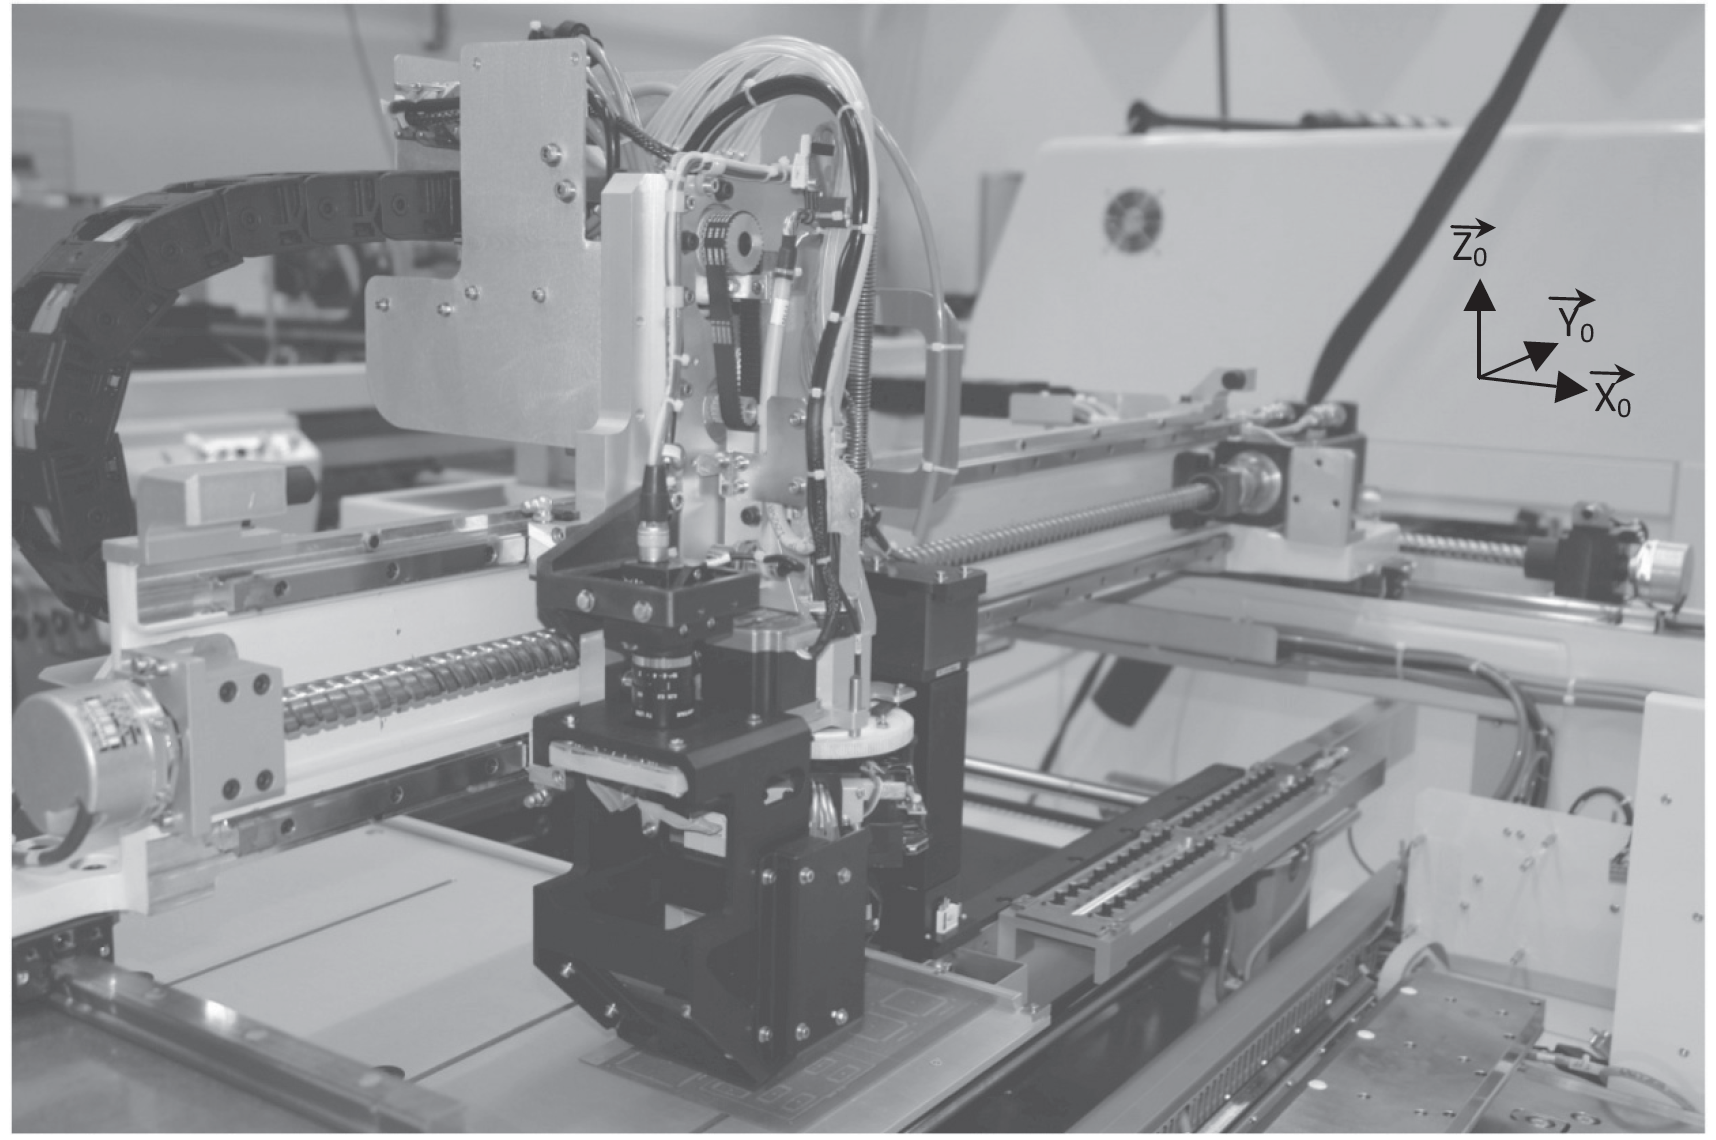
\includegraphics[width=.7\linewidth]{images/axe_y_photo}
}%figues de la page de garde


\def\xxpied{%
Cycle 06 -- Modélisation mécanique -- Énergétique\\% afin de valider leurs performances.\\
Chapitre 1 -- \xxactivite%
}

\setcounter{secnumdepth}{5}
%---------------------------------------------------------------------------

\usepackage{pgfplots}
\begin{document}
\def\pathfig{images}
%\chapterimage{png/Fond_Cin}
\pagestyle{empty}


%%%%%%%% PAGE DE GARDE COURS
\ifcours
% ==== BANDEAU DES TITRES ==== 
\begin{tikzpicture}[remember picture,overlay]
\node at (current page.north west)
{\begin{tikzpicture}[remember picture,overlay]
\node[anchor=north west,inner sep=0pt] at (0,0) {\includegraphics[width=\paperwidth]{\thechapterimage}};
\draw[anchor=west] (-2cm,-8cm) node [line width=2pt,rounded corners=15pt,draw=ocre,fill=white,fill opacity=0.6,inner sep=40pt]{\strut\makebox[22cm]{}};
\draw[anchor=west] (1cm,-8cm) node {\huge\sffamily\bfseries\color{black} %
\begin{minipage}{1cm}
\rotatebox{90}{\LARGE\sffamily\textsc{\color{ocre}\textbf{\xxnumpartie}}}
\end{minipage} \hfill
\begin{minipage}[c]{14cm}
\begin{titrepartie}
\begin{flushright}
\renewcommand{\baselinestretch}{1.1} 
\Large\sffamily\textsc{\textbf{\xxpartie}}
\renewcommand{\baselinestretch}{1} 
\end{flushright}
\end{titrepartie}
\end{minipage} \hfill
\begin{minipage}[c]{3.5cm}
{\large\sffamily\textsc{\textbf{\color{ocre} \discipline}}}
\end{minipage} 
 };
\end{tikzpicture}};
\end{tikzpicture}
% ==== FIN BANDEAU DES TITRES ==== 


% ==== ONGLET 
\begin{tikzpicture}[overlay]
\node[shape=rectangle, 
      rounded corners = .25 cm,
	  draw= ocre,
	  line width=2pt, 
	  fill = ocre!10,
	  minimum width  = 2.5cm,
	  minimum height = 3cm,] at (18.3cm,0) {};
\node at (17.7cm,0) {\rotatebox{90}{\textbf{\Large\color{ocre}{\classe}}}};
%{};
\end{tikzpicture}
% ==== FIN ONGLET 


\vspace{3.5cm}

\begin{tikzpicture}[remember picture,overlay]
\draw[anchor=west] (-2cm,-6cm) node {\huge\sffamily\bfseries\color{black} %
\begin{minipage}{2cm}
\begin{center}
\LARGE\sffamily\textsc{\color{ocre}\textbf{\xxactivite}}
\end{center}
\end{minipage} \hfill
\begin{minipage}[c]{15cm}
\begin{titrechapitre}
\renewcommand{\baselinestretch}{1.1} 
\Large\sffamily\textsc{\textbf{\xxnumchapitre}}

\Large\sffamily\textsc{\textbf{\xxchapitre}}
\vspace{.5cm}

\renewcommand{\baselinestretch}{1} 
\normalsize\normalfont
\xxcompetences
\end{titrechapitre}
\end{minipage}  };
\end{tikzpicture}
\vfill

\begin{flushright}
\begin{minipage}[c]{.3\linewidth}
\begin{center}
\xxfigures
\end{center}
\end{minipage}\hfill
\begin{minipage}[c]{.6\linewidth}
\startcontents
%\printcontents{}{1}{}
\printcontents{}{1}{}
\end{minipage}
\end{flushright}

\begin{tikzpicture}[remember picture,overlay]
\draw[anchor=west] (4.5cm,-.7cm) node {
\begin{minipage}[c]{.2\linewidth}
\begin{flushright}

\includegraphics[width=2cm]{logoCC}
\end{flushright}
\end{minipage}
\begin{minipage}[c]{.2\linewidth}
\textsl{\xxauteur} \\
\textsl{\classe}
\end{minipage}
 };
\end{tikzpicture}

\newpage
\pagestyle{fancy}

%\newpage
%\pagestyle{fancy}

\else
\fi
%% FIN PAGE DE GARDE DES COURS

%%%%%%%% PAGE DE GARDE TD
\iftd
%\begin{tikzpicture}[remember picture,overlay]
%\node at (current page.north west)
%{\begin{tikzpicture}[remember picture,overlay]
%\draw[anchor=west] (-2cm,-3.25cm) node [line width=2pt,rounded corners=15pt,draw=ocre,fill=white,fill opacity=0.6,inner sep=40pt]{\strut\makebox[22cm]{}};
%\draw[anchor=west] (1cm,-3.25cm) node {\huge\sffamily\bfseries\color{black} %
%\begin{minipage}{1cm}
%\rotatebox{90}{\LARGE\sffamily\textsc{\color{ocre}\textbf{\xxnumpartie}}}
%\end{minipage} \hfill
%\begin{minipage}[c]{13.5cm}
%\begin{titrepartie}
%\begin{flushright}
%\renewcommand{\baselinestretch}{1.1} 
%\Large\sffamily\textsc{\textbf{\xxpartie}}
%\renewcommand{\baselinestretch}{1} 
%\end{flushright}
%\end{titrepartie}
%\end{minipage} \hfill
%\begin{minipage}[c]{3.5cm}
%{\large\sffamily\textsc{\textbf{\color{ocre} \discipline}}}
%\end{minipage} 
% };
%\end{tikzpicture}};
%\end{tikzpicture}

%%%%%%%%%% PAGE DE GARDE TD %%%%%%%%%%%%%%%
%\begin{tikzpicture}[overlay]
%\node[shape=rectangle, 
%      rounded corners = .25 cm,
%	  draw= ocre,
%	  line width=2pt, 
%	  fill = ocre!10,
%	  minimum width  = 2.5cm,
%	  minimum height = 2.5cm,] at (18.5cm,0) {};
%\node at (17.7cm,0) {\rotatebox{90}{\textbf{\Large\color{ocre}{\classe}}}};
%%{};
%\end{tikzpicture}

% PARTIE ET CHAPITRE
%\begin{tikzpicture}[remember picture,overlay]
%\draw[anchor=west] (-1cm,-2.1cm) node {\large\sffamily\bfseries\color{black} %
%\begin{minipage}[c]{15cm}
%\begin{flushleft}
%\xxnumchapitre \\
%\xxchapitre
%\end{flushleft}
%\end{minipage}  };
%\end{tikzpicture}

% BANDEAU EXO
\iflivret % SI LIVRET
\begin{tikzpicture}[remember picture,overlay]
\draw[anchor=west] (-2cm,-3.3cm) node {\huge\sffamily\bfseries\color{black} %
\begin{minipage}{5cm}
\begin{center}
\LARGE\sffamily\color{ocre}\textbf{\textsc{\xxactivite}}

\begin{center}
\xxfigures
\end{center}

\end{center}
\end{minipage} \hfill
\begin{minipage}[c]{12cm}
\begin{titrechapitre}
\renewcommand{\baselinestretch}{1.1} 
\large\sffamily\textbf{\textsc{\xxtitreexo}}

\small\sffamily{\textbf{\textit{\color{black!70}\xxsourceexo}}}
\vspace{.5cm}

\renewcommand{\baselinestretch}{1} 
\normalsize\normalfont
\xxcompetences
\end{titrechapitre}
\end{minipage}};
\end{tikzpicture}
\else % ELSE NOT LIVRET
\begin{tikzpicture}[remember picture,overlay]
\draw[anchor=west] (-2cm,-4.5cm) node {\huge\sffamily\bfseries\color{black} %
\begin{minipage}{5cm}
\begin{center}
\LARGE\sffamily\color{ocre}\textbf{\textsc{\xxactivite}}

\begin{center}
\xxfigures
\end{center}

\end{center}
\end{minipage} \hfill
\begin{minipage}[c]{12cm}
\begin{titrechapitre}
\renewcommand{\baselinestretch}{1.1} 
\large\sffamily\textbf{\textsc{\xxtitreexo}}

\small\sffamily{\textbf{\textit{\color{black!70}\xxsourceexo}}}
\vspace{.5cm}

\renewcommand{\baselinestretch}{1} 
\normalsize\normalfont
\xxcompetences
\end{titrechapitre}
\end{minipage}};
\end{tikzpicture}

\fi

\else   % FIN IF TD
\fi


%%%%%%%% PAGE DE GARDE FICHE
\iffiche
\begin{tikzpicture}[remember picture,overlay]
\node at (current page.north west)
{\begin{tikzpicture}[remember picture,overlay]
\draw[anchor=west] (-2cm,-2.25cm) node [line width=2pt,rounded corners=15pt,draw=ocre,fill=white,fill opacity=0.6,inner sep=40pt]{\strut\makebox[22cm]{}};
\draw[anchor=west] (1cm,-2.25cm) node {\huge\sffamily\bfseries\color{black} %
\begin{minipage}{1cm}
\rotatebox{90}{\LARGE\sffamily\textsc{\color{ocre}\textbf{\xxnumpartie}}}
\end{minipage} \hfill
\begin{minipage}[c]{14cm}
\begin{titrepartie}
\begin{flushright}
\renewcommand{\baselinestretch}{1.1} 
\large\sffamily\textsc{\textbf{\xxpartie} \\} 

\vspace{.2cm}

\normalsize\sffamily\textsc{\textbf{\xxnumchapitre -- \xxchapitre}}
\renewcommand{\baselinestretch}{1} 
\end{flushright}
\end{titrepartie}
\end{minipage} \hfill
\begin{minipage}[c]{3.5cm}
{\large\sffamily\textsc{\textbf{\color{ocre} \discipline}}}
\end{minipage} 
 };
\end{tikzpicture}};
\end{tikzpicture}

\iflivret
\begin{tikzpicture}[overlay]
\node[shape=rectangle, 
      rounded corners = .25 cm,
	  draw= ocre,
	  line width=2pt, 
	  fill = ocre!10,
	  minimum width  = 2.5cm,
	  minimum height = 2.5cm,] at (18.5cm,1.1cm) {};
\node at (17.9cm,1.1cm) {\rotatebox{90}{\textsf{\textbf{\large\color{ocre}{\classe}}}}};
%{};
\end{tikzpicture}
\else
\begin{tikzpicture}[overlay]
\node[shape=rectangle, 
      rounded corners = .25 cm,
	  draw= ocre,
	  line width=2pt, 
	  fill = ocre!10,
	  minimum width  = 2.5cm,
%	  minimum height = 2.5cm,] at (18.5cm,1.1cm) {};
	  minimum height = 2.5cm,] at (18.6cm,0cm) {};
\node at (18cm,0cm) {\rotatebox{90}{\textsf{\textbf{\large\color{ocre}{\classe}}}}};
%{};
\end{tikzpicture}

\fi

\else
\fi



\vspace{4.5cm}
\pagestyle{fancy}
\thispagestyle{plain}

\def\columnseprulecolor{\color{ocre}}
\setlength{\columnseprule}{0.4pt} 

\def\pathfig{images}

\ifprof
\begin{multicols}{2}
\else
\begin{multicols}{2}
\fi


\section*{Exercice 1 -- Trains d'engrenages simples}
\setcounter{exo}{0}

\ifprof
\else
Soit le train d'engrenages suivant. 
\begin{center}
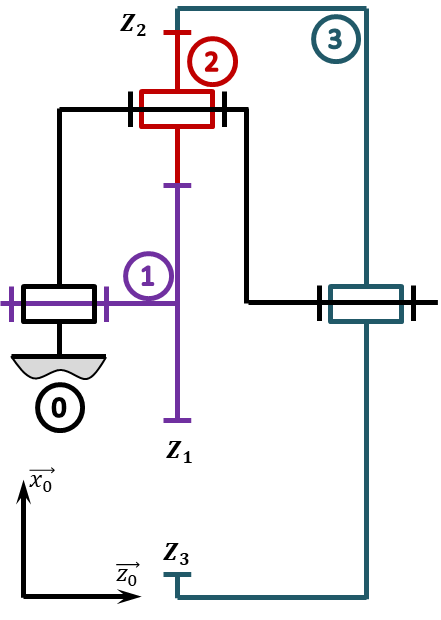
\includegraphics[width=.7\linewidth]{images/TrainSimple_01}
\end{center}
\fi

\subparagraph{}
\textit{Déterminer $\dfrac{\omega_{3/0}}{\omega_{1/0}}$ en fonction du nombre de dents des roues dentées.}
\ifprof
\begin{corrige}
On a $\dfrac{\omega_{3/0}}{\omega_{1/0}}=-\dfrac{Z_1}{Z_3}$.
\end{corrige}
\else
\fi

\subparagraph{}
\textit{Donner une relation géométrique entre $Z_1$, $Z_2$ et $Z_3$ permettant de garantir le fonctionnement du train d'engrenages. }
\ifprof
\begin{corrige}
On a $Z_3 = 2Z_2 + Z_1$.
\end{corrige}
\else
\fi



\ifprof
\else
Soit le train d'engrenages suivant. 
\begin{center}
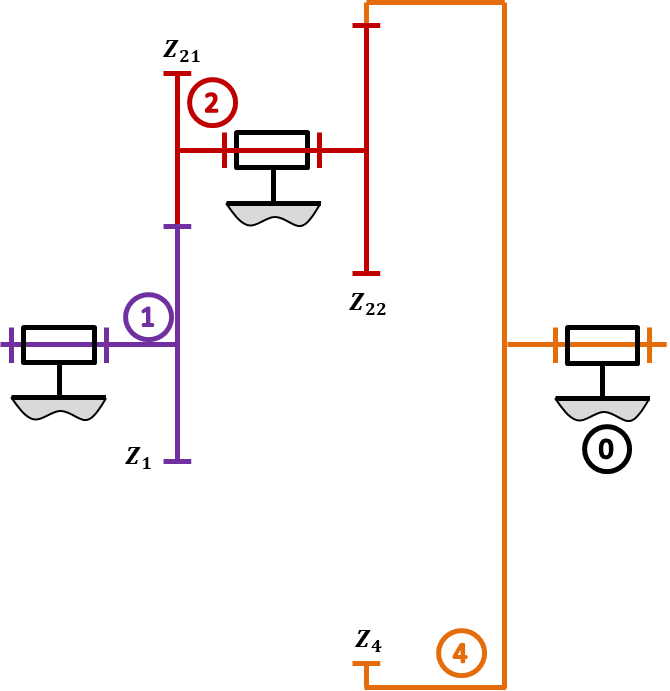
\includegraphics[width=.7\linewidth]{images/TrainSimple_02}
\end{center}
\fi

\subparagraph{}
\textit{Déterminer $\dfrac{\omega_{4/0}}{\omega_{1/0}}$ en fonction du nombre de dents des roues dentées.}
\ifprof
\begin{corrige}
On a $\dfrac{\omega_{4/0}}{\omega_{1/0}}=-\dfrac{Z_1Z_{22}}{Z_4Z_{21}}$.
\end{corrige}
\else
\fi

\subparagraph{}
\textit{Donner une relation géométrique entre $Z_1$, $Z_{21}$, $Z_{22}$ et $Z_4$ permettant de garantir le fonctionnement du train d'engrenages. }
\ifprof
\begin{corrige}
On a $Z_1+Z_{21}+Z_{22}= Z_4$.
\end{corrige}
\else
\fi



\ifprof
\else
Soit le train d'engrenages suivant. 
\begin{center}
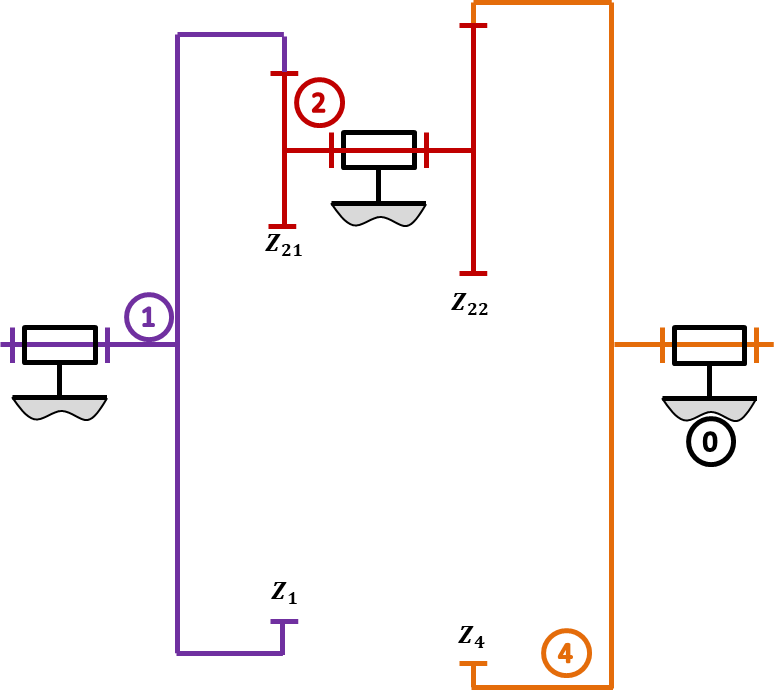
\includegraphics[width=.7\linewidth]{images/TrainSimple_03}
\end{center}
\fi


\subparagraph{}
\textit{Déterminer $\dfrac{\omega_{4/0}}{\omega_{1/0}}$ en fonction du nombre de dents des roues dentées.}
\ifprof
\begin{corrige}
On a $\dfrac{\omega_{4/0}}{\omega_{1/0}}=\dfrac{Z_1Z_{22}}{Z_4Z_{21}}$.
\end{corrige}
\else
\fi


\ifprof
\else
Soit le train d'engrenages suivant. 
\begin{center}
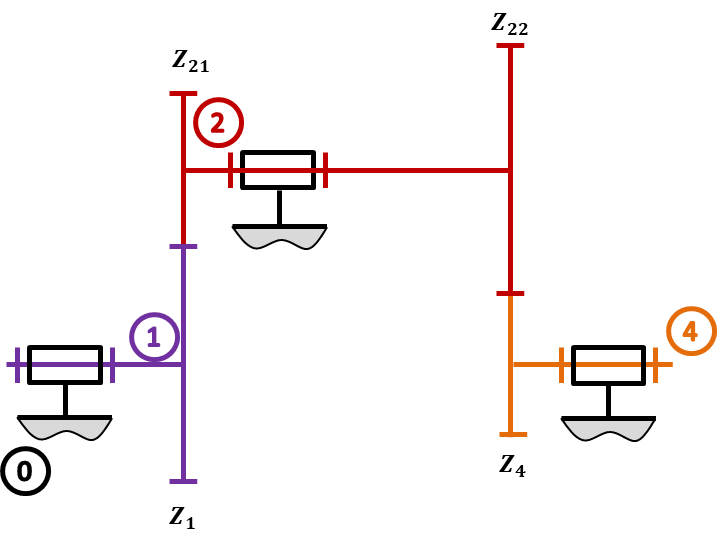
\includegraphics[width=.7\linewidth]{images/TrainSimple_04}
\end{center}
\fi


\subparagraph{}
\textit{Déterminer $\dfrac{\omega_{4/0}}{\omega_{1/0}}$ en fonction du nombre de dents des roues dentées.}
\ifprof
\begin{corrige}
On a $\dfrac{\omega_{4/0}}{\omega_{1/0}}=\dfrac{Z_1Z_{22}}{Z_4Z_{21}}$.
\end{corrige}
\else
\fi




%\section*{Exercice 2 -- Train d'engrenages (cheville NAO)}
%\setcounter{exo}{0}
%
%
%\ifprof
%\else
%NAO est un robot humanoïde conçu par la société française Aldebaran. À l'origine il a été conçu comme prototype du robot Romeo, destiné à être au service des personnes. NAO est utilisé à l'heure actuelle dans la recherche en robotique et dans des domaines pédagogiques. 
%\begin{obj}
%On s'intéresse ici à la cheville NAO. On cherche à savoir si, à partir du moteur retenu par le constructeur, la chaîne de transmission de puissance permet de vérifier les exigences suivantes : 
%\begin{itemize}
%\item exigence 1.1.1.1 : la vitesse de roulis doit être inférieure à \SI{42}{tr/min};
%\item exigence 1.1.1.2 : la vitesse de tangage doit être inférieure à \SI{60}{tr/min}.
%\end{itemize}
%
%\end{obj}
%
%
%
%\begin{center}
%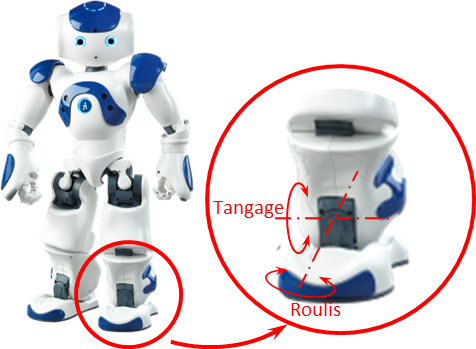
\includegraphics[width=.7\linewidth]{images/nao_01}
%\end{center}
%
%La fréquence de rotation des moteurs permettant chacun des deux mouvements est de \SI{8300}{tr/min}.
%
%Pour la chaîne de transmission de tangage on donne  le nombre de dents et le module de chaque roue dentée : 
%\begin{itemize}
%\item pignon moteur : $Z_m=20$, $M_m=0,3$;
%\item grand pignon 1 : $Z_1 = 80$, $M_1=0,3$;
%\item petit pignon 1 : $Z_1' = 25$, $M_1'=0,4$;
%\item grand pignon 2 : $Z_2 = 47$, $M_2=0,4$;
%\item petit pignon 2 : $Z_2' = 12$, $M_2'=0,4$;
%\item grand pignon 3 : $Z_3 = 58$, $M_3=0,4$;
%\item petit pignon 3 : $Z_3' = 10$, $M_3'=0,7$;
%\item roue de sortie : $Z_T = 36$, $M_T=0,7$.
%\end{itemize}
%
%\begin{center}
%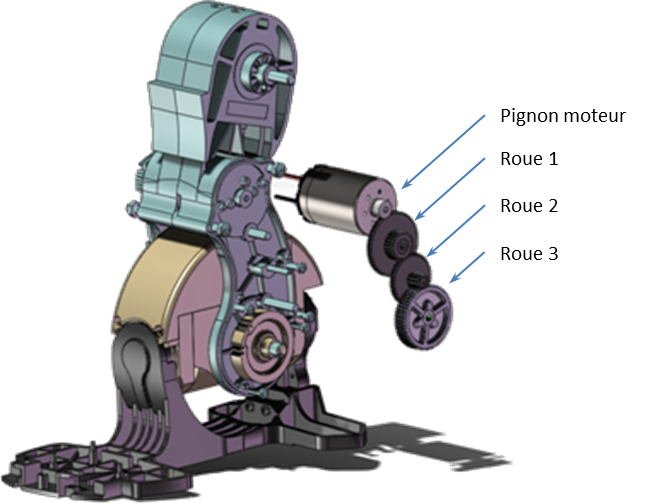
\includegraphics[width=.95\linewidth]{images/nao_02}
%\end{center}
%
%Pour la chaîne de transmission du roulis on donne le nombre de dents et le module de chaque roue dentée : 
%\begin{itemize}
%\item pignon moteur : $Z_m=13$, $M_m=0,3$;
%\item grand pignon 1 : $Z_1 = 80$, $M_1=0,3$;
%\item petit pignon 1 : $Z_1' = 25$, $M_1'=0,4$;
%\item grand pignon 2 : $Z_2 = 47$, $M_2=0,4$;
%\item petit pignon 2 : $Z_2' = 12$, $M_2'=0,4$;
%\item grand pignon 3 : $Z_3 = 58$, $M_3=0,4$;
%\item petit pignon 3 : $Z_3' = 10$, $M_3'=0,7$;
%\item roue de sortie 3 : $Z_R = 36$, $M_R=0,7$.
%\end{itemize}
%
%
%
%\begin{center}
%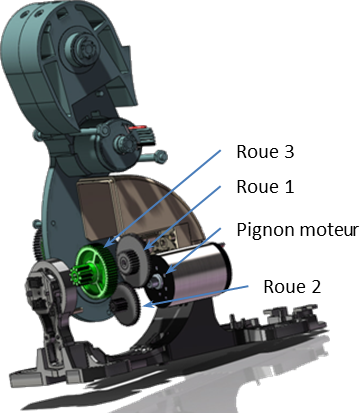
\includegraphics[width=.8\linewidth]{images/nao_03}
%\end{center}
%\fi
%
%
%
%\subparagraph{}
%\textit{Quels doivent être les rapports de réductions des transmissions par engrenage afin de respecter les exigences 1.1.1.1 et 1.1.1.2 ?}
%\ifprof
%\begin{corrige}
%D'après le diagramme de définition des blocs et le diagramme des exigences, les rapports de transmission doivent être : 
%\begin{itemize}
%\item pour l'axe de tangage : $\dfrac{N_{\text{moteur}}}{N_{\text{Tangage}}}=138,33$ au minimum; 
%\item pour l'axe de roulis :  $\dfrac{N_{\text{moteur}}}{N_{\text{Roulis}}}= 197,61$ au minimum.
%\end{itemize}
%\end{corrige}
%\else
%\fi
%
%
%\ifprof
%\subparagraph{}
%\textit{Dans le cas de l'axe de tangage, remplir le tableau suivant :}
%\begin{corrige} ~\\
%\begin{center}
%\begin{tabular}{|p{1.7cm}|c|c|p{1.3cm}|}
%\hline
%Roue dentée & Module & Nb dents & Diamètre (mm)\\
%\hline
%Pignon 03 20 & 0,3 &20        & 6		\\ \hline
%Mobile Inf1 Roue & 0,3 & 80  & 24 	\\ \hline 
%Mobile Inf1 Pignon & 0,4 & 25 & 10	\\ \hline
%Mobile Inf2 Roue & 0,4 & 47   & 18,8	\\ \hline
%Mobile Inf2 Pignon & 0,4 & 12 & 4,8	\\ \hline
%Mobile Inf4 Roue & 0,4 & 58   & 23,2	\\ \hline
%Mobile Inf4 Pignon & 0,7 & 10 & 7	\\ \hline
%Roue de sortie & 0,7 & 36      & 25,2 \\ \hline
%\end{tabular}
%\end{center}
%\end{corrige}
%\else
%\fi
%
%\subparagraph{}
%\textit{Dans le cas de l'axe de tangage, déterminer le diamètre de chaque roue dentée.}
%%
%%\begin{center}
%%\begin{tabular}{|l|c|c|c|}
%%\hline
%%Roue dentée & Module & Nb dents & Diamètre \\
%%\hline
%%& && \\ 
%%Pignon 03 20 & && \\ 
%%&& & \\ \hline
%%&& & \\ 
%%Mobile Inf1 Roue & && \\ 
%%&& & \\ \hline
%%&& & \\ 
%%Mobile Inf1 Pignon & && \\ 
%%&& & \\ \hline
%%&& & \\ 
%%Mobile Inf2 Roue & && \\ 
%%&& & \\ \hline
%%&& & \\ 
%%Mobile Inf2 Pignon & && \\ 
%%&& & \\ \hline
%%&& & \\ 
%%Mobile Inf4 Roue & && \\ 
%%&& & \\ \hline
%%&& & \\ 
%%Mobile Inf4 Pignon & && \\ 
%%&& & \\ \hline
%%&& & \\ 
%%Roue de sortie & && \\
%%&& & \\ 
%%\hline
%%\end{tabular}
%%\end{center}
%%\fi
%%
%%
%\subparagraph{}
%\textit{Dans le cas de l'axe de tangage, réaliser le schéma cinématique minimal.}
%\ifprof
%\begin{corrige}
%\end{corrige}
%\else
%\fi
%
%\subparagraph{}
%\textit{Calculer le rapport de transmission de la chaîne de transmission de l'axe de tangage ? L'exigence 1.1.1.2 est-elle respectée ? Si non, quelle(s) solution(s) de remédiation pourrait-on proposer ?}
%\ifprof
%\begin{corrige}
%$$
%R_T = (-1)^n \dfrac{80\cdot 47 \cdot 58 \cdot 36}{20\cdot 25\cdot 12 \cdot 10 } = 130,85
%$$
%
%Ceci est inférieur à ce qui est préconisé par le cahier des charges. 
%
%Pour respecter le cahier des charges, on peut :
%\begin{itemize}
%\item choisir un autre moteur;
%\item changer le nombre de dents d'une des roues. Il suffirait pour cela que,  par exemple, la roue de sortie comporte 39 dents. 
%\end{itemize}
%\end{corrige}
%\else
%\fi
%
%\subparagraph{}
%\textit{Calculer le rapport de transmission de la chaîne de transmission de l'axe de roulis ? L'exigence 1.1.1.1 est-elle respectée ? Si non, quelle(s) solution(s) de remédiation pourrait-on proposer ?}
%\ifprof
%\begin{corrige}
%Le rapport de transmission du second train est de 201,3 ce qui est compatible avec le cahier des charges.
%\end{corrige}
%\else
%\fi


\section*{Exercice 3 -- Réducteur de roue motrice de chariot élévateur}
\textit{D'après Florestan Mathurin.}
\setcounter{exo}{0}

\ifprof
\else

On s’intéresse au réducteur équipant la roue arrière motrice et directionnelle d’un chariot élévateur de manutention automoteur à conducteur non porté. 



\begin{center}
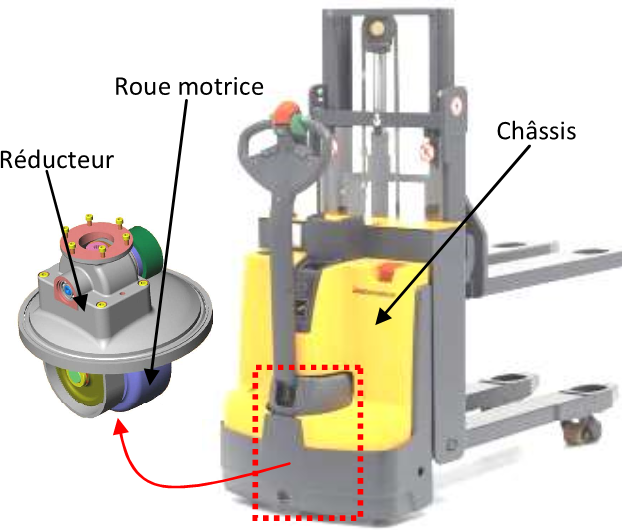
\includegraphics[width=.95\linewidth]{images/char_01}
\end{center}


\textbf{Données }: $z_{27} = \SI{16}{dents}$, $z_{35} = \SI{84}{dents}$, $z_{5} = \SI{14}{dents}$, $z_{11} = \SI{56}{dents}$, $z_{16} = \SI{75}{dents}$. 

\fi

\subparagraph{}
\textit{Identifier les classes d’équivalence cinématique sur le dessin d’ensemble. }
\ifprof
\begin{corrige}

\end{corrige}
\else
\begin{center}
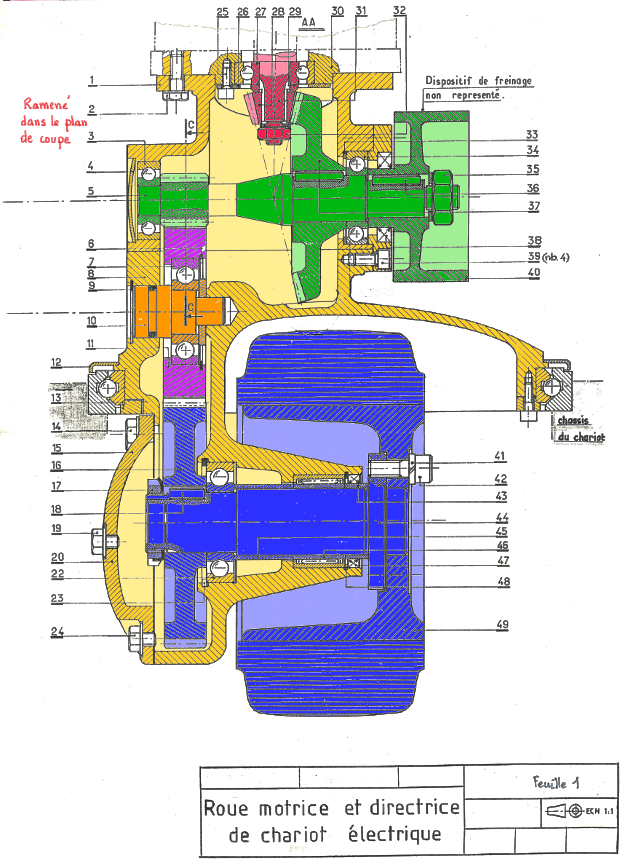
\includegraphics[width=\linewidth]{images/char_02}
\end{center}

\fi



\subparagraph{}
\textit{ Construire le schéma cinématique du réducteur dans le même plan que le dessin.}
\ifprof
\begin{corrige}
\begin{center}
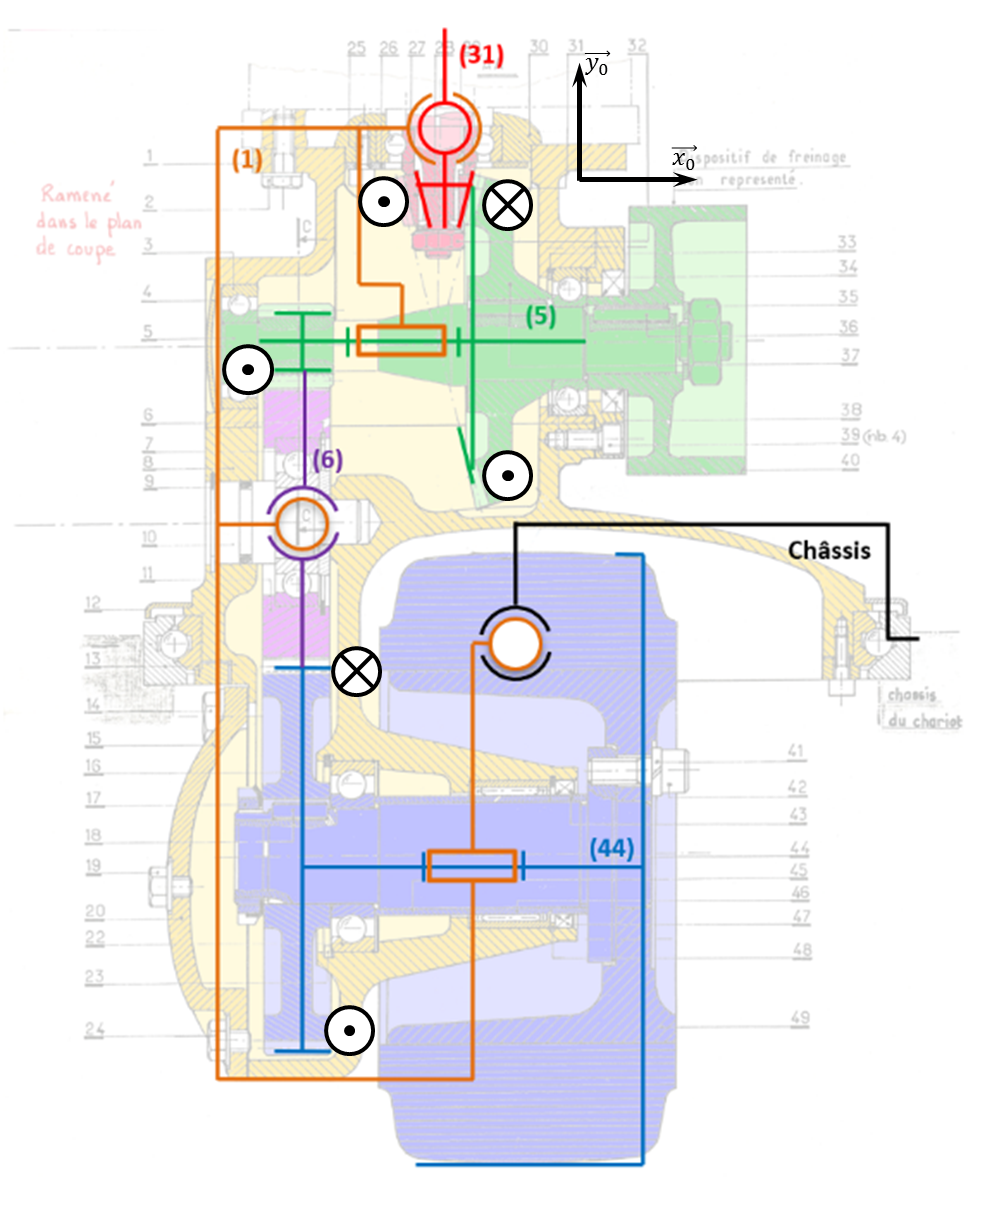
\includegraphics[width=\linewidth]{images/char_cor_01_BIS}
\end{center}
\end{corrige}
\else
\fi
\subparagraph{}
\textit{Compléter le tableau donnant les caractéristiques des roues et pignons.}
\ifprof
\begin{corrige}
\footnotesize
\begin{center}
\begin{tabular}{|c|c|c|c|}
\hline
Repère de  & Module  & Nombre & Diamètre primitif  \\
la roue & $m$ (mm) & de dents $Z$ & $D$ (mm) \\
\hline
\hline
27 & 1,5 &16 & 24\\ \hline
35 & 1,5 &84 & 126\\ \hline
5   &1,5 &14 & 21\\ \hline
11 & 1,5 & 56 & 84 \\ \hline
16 &  1,5&  75& 112,5\\ \hline

\end{tabular}
\end{center}

\normalsize
\end{corrige}
\else
\footnotesize
\begin{center}
\begin{tabular}{|c|c|c|c|}
\hline
Repère de  & Module  & Nombre & Diamètre primitif  \\
la roue & $m$ (mm) & de dents $Z$ & $D$ (mm) \\
\hline
\hline
27 & & & \\ \hline
35 & 1,5& & \\ \hline
5& & & \\ \hline
11& 1,5 & & \\ \hline
16& & & \\ \hline

\end{tabular}
\end{center}

\normalsize
\fi



\subparagraph{}
\textit{Après avoir proposé un paramétrage, indiquer dans quel sens tourne la roue si le moteur 28 (31) tourne dans le sens positif.}

\ifprof
\begin{corrige}
Voir figure précédente. Si le moteur tourne dans le sens positif, la roue tourne dans le sens négatif. 
\end{corrige}
\else
\fi

\subparagraph{}
\textit{Pour une vitesse de \SI{1500}{tr/min} en sortie de moteur, déterminer la vitesse de rotation de la roue. Le diamètre de la roue est de \SI{150}{mm}. Quelle est la vitesse du véhicule ? }
\ifprof
\begin{corrige}
Le rapport de réduction de la transmission est le suivant : 
$k=\dfrac{Z_{27} Z_{5} Z_{11} }{Z_{35} Z_{11} Z_{16}} = \dfrac{16\cdot 14}{84\cdot 75} =0,0355 $

La vitesse de rotation de la roue est donc de $\SI{53,33}{tr.min^{-1}}$ soit \SI{5,59}{rad.s^{-1}}. 
On en déduit la vitesse du véhicule : $5,59 \times 0,15 = \SI{0,84}{m.s^{-1}}\simeq \SI{3}{km.h^{-1}}$.

\end{corrige}
\else
\fi

\section*{Exercice 4 -- Train épicycloïdal -- Type 1 -- Sécateur Pellenc}
\setcounter{exo}{0}
\textit{D'après ressources de Florestan Mathurin.}

\ifprof
\else

\begin{obj}~\\
Vérifier les performances d'un réducteur.
\end{obj}


La période de taille de la vigne dure 2 mois environ. Les viticulteurs coupent 9 à 10 heures par jour. Ils répètent donc le même geste des millions de fois avec un sécateur. Les sociétés réalisant le du matériel agricole ont imaginé un sécateur électrique capable de réduire la fatigue de la main et du bras tout en laissant au viticulteur la commande de la coupe et sa liberté de mouvement. Le sécateur développé par la société Pellenc permet notamment de réaliser 60 coupes de diamètre 22 mm par minute. L’ensemble sécateur Pellenc est constitué d’un sécateur électronique, d’une mallette source d’énergie, d’une sacoche avec harnais et ceinture et d’un chargeur de batterie.

%
%\begin{center}
% 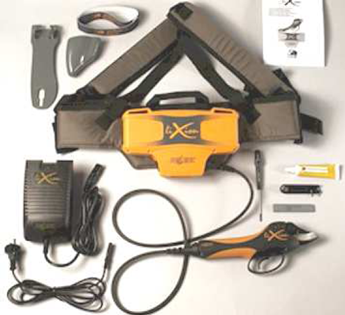
\includegraphics[width=.95\linewidth]{images/secateur1}
%\end{center}


Lorsque l’utilisateur appuie sur la gâchette, le moteur transmet par l’intermédiaire d’un réducteur à train épicycloïdal un mouvement de rotation à la vis à billes. L’écrou se déplace en translation par rapport à la vis et par l’intermédiaire d’une biellette met en rotation la lame mobile générant ainsi le mouvement de coupe. 

\begin{center}
 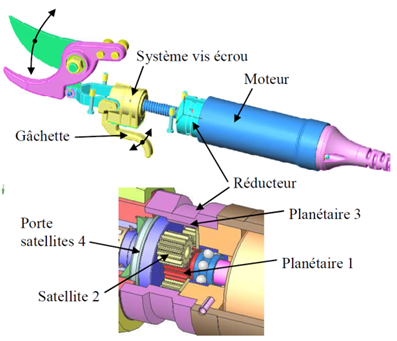
\includegraphics[width=.95\linewidth]{images/secateur2}
\end{center}




Le moteur tourne à la vitesse de rotation $N_1=1\,400\;\text{tr/min}$ le (le rotor est lié au planétaire 1). La vis à billes liée au porte-satellite 4 tourne à la vitesse de rotation $N_4=350^; \text{tr/min}$. On note $Z_1$ le nombre dents du planétaire 1, $Z_2$ celui du satellite 2 et $Z_3$ celui de la couronne liée au bâti.

\begin{center}
 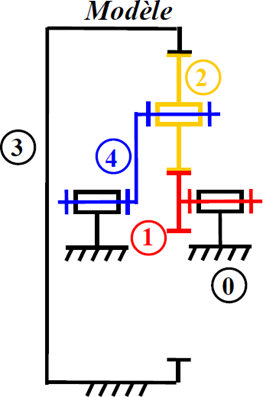
\includegraphics[width=.6\linewidth]{images/secateur3}
\end{center}

\fi

\subparagraph{}
\textit{Déterminer le rapport de réduction du train épicycloïdal $\dfrac{\omega(4/0)}{\omega(1/0)}$ en fonction de $Z_1$ et $Z_3$.}
 \ifprof
 \begin{corrige}
 On écrit le rapport des vitesses par rapport au porte-satellite 4 : $\dfrac{\omega(3/4)}{\omega(1/4)} = - \dfrac{Z_1}{Z_3}$.
 
 En réalisant une décomposition du taux de rotation : $\dfrac{\omega(3/0)+\omega(0/4)}{\omega(1/0)+\omega(0/4)} = \dfrac{-\omega(4/0)}{\omega(1/0)-\omega(4/0)}= \dfrac{-\omega(4/0)}{\omega(1/0)-\omega(4/0)} =- \dfrac{Z_1}{Z_3}$ $\Leftrightarrow \dfrac{\omega(4/0)}{\omega(1/0)-\omega(4/0)} = \dfrac{Z_1}{Z_3} $
 $\Leftrightarrow {\omega(4/0)} = \dfrac{Z_1}{Z_3} \omega(1/0)-\dfrac{Z_1}{Z_3} \omega(4/0)$
 $\Leftrightarrow {\omega(4/0)} \left(1+\dfrac{Z_1}{Z_3} \right)= \dfrac{Z_1}{Z_3} \omega(1/0)$
 $\Leftrightarrow \dfrac{\omega(4/0)}{\omega(1/0)}=  \dfrac{Z_1}{Z_1+Z_3} $.
 \end{corrige}
 \else
 \fi
 
\subparagraph{}
\textit{Faire l’application numérique et déterminer une relation entre $Z_1$ et $Z_3$. Sachant que $Z_1=19$ en déduire $Z_3$.}
 \ifprof
 \begin{corrige}
 On a $\dfrac{N_4}{N_1}=\dfrac{Z_1}{Z_1+Z_3} $ $\Leftrightarrow Z_3=\dfrac{Z_1 N_1}{N_4} -  Z_1 $ 
 $\Leftrightarrow Z_3=\dfrac{19 \times 1400}{350} -  19 = \SI{57}{dents}$.
 \end{corrige}
 \else
 \fi
 
\subparagraph{}
\textit{Sachant que les roues dentées du train ont les mêmes modules, déterminer une relation géométrique entre les diamètres des éléments dentés $d_1$, $d_2$, $d_3$ puis en déduire une relation entre $Z_2$, $Z_1$, $Z_3$ (condition d’entraxe). Calculer la valeur de $Z_2$.}

 \ifprof
 \begin{corrige}
 On a $R_1+2R_2 = R_3$ $\Leftrightarrow Z_1+2Z_2 = Z_3$ $\Leftrightarrow Z_2 = \dfrac{Z_3- Z_1}{2}=\dfrac{57-19}{2}=\SI{19}{dents}$.
 \end{corrige}
 \else
 \fi



\ifprof
\newpage
\else
\fi

\section*{Exercice 5 -- Trains épicycloïdaux}
\setcounter{exo}{0}


Soit le train épicycloïdal suivant. 

\begin{center}
 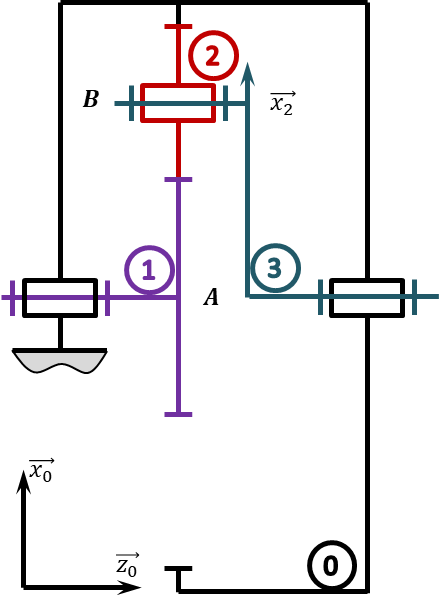
\includegraphics[width=.6\linewidth]{images/TrainEpi_01.png}
\end{center}



\subparagraph{}
\textit{Déterminer le rapport de réduction $\dfrac{\omega_{30}}{\omega_{10}}$.}
 \ifprof
 \begin{corrige}
 
 En bloquant le porte satellite, on a : $\dfrac{\omega_{03}}{\omega_{13}}=-\dfrac{Z_1}{Z_0}$. On a donc, 
$\dfrac{\omega_{03}}{\omega_{10}+\omega_{03}}=-\dfrac{Z_1}{Z_0}$

$\Leftrightarrow \dfrac{\omega_{30}}{\omega_{30}-\omega_{10}}=-\dfrac{Z_1}{Z_0}$
$\Leftrightarrow \omega_{30}=-\dfrac{Z_1}{Z_0} \omega_{30}+\dfrac{Z_1}{Z_0}\omega_{10} $
$\Leftrightarrow \omega_{30}\left( 1+\dfrac{Z_1}{Z_0} \right)=\dfrac{Z_1}{Z_0}\omega_{10} $
$\Leftrightarrow \omega_{30}=\dfrac{Z_1}{Z_0+Z_1}\omega_{10} $
 \end{corrige}
 \else
 \fi



Soit le train épicycloïdal suivant. 

\begin{center}
 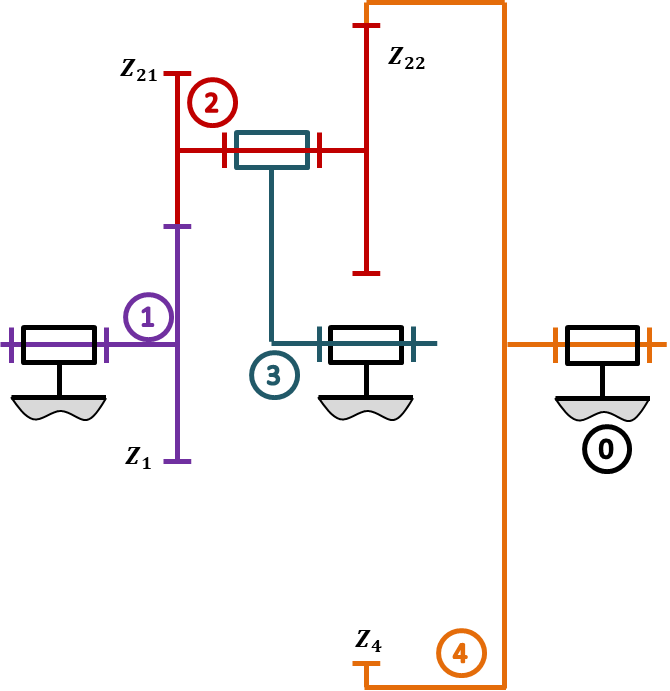
\includegraphics[width=.6\linewidth]{images/TrainEpi_02.png}
\end{center}




\subparagraph{}
\textit{Déterminer $\omega_{40}$ en fonction de  $\omega_{30}$ et $\omega_{10}$.}
 \ifprof
 \begin{corrige}
 
 En bloquant le porte satellite, on a : $\dfrac{\omega_{43}}{\omega_{13}}=-\dfrac{Z_{1}Z_{22}}{Z_{21}Z_{4}}$.
  On a donc, 
  $\dfrac{\omega_{40}+\omega_{03}}{\omega_{10}+\omega_{03}}=-\dfrac{Z_{1}Z_{22}}{Z_{21}Z_{4}}$

  $\Leftrightarrow \omega_{40}+\omega_{03}=-\dfrac{Z_{1}Z_{22}}{Z_{21}Z_{4}}\left( \omega_{10}+\omega_{03} \right)$
  
  $\Leftrightarrow \omega_{40}=-\dfrac{Z_{1}Z_{22}}{Z_{21}Z_{4}}\left( \omega_{10}+\omega_{03} \right)-\omega_{03}$
  
    $\Leftrightarrow \omega_{40}=-\dfrac{Z_{1}Z_{22}}{Z_{21}Z_{4}}\left( \omega_{10}+\omega_{03} \right)+\omega_{30}$
    
      $\Leftrightarrow \omega_{40}=-\dfrac{Z_{1}Z_{22}}{Z_{21}Z_{4}}\omega_{10}+\omega_{30}\left( 1+\dfrac{Z_{1}Z_{22}}{Z_{21}Z_{4}} \right)$

 \end{corrige}
 \else
 \fi




\subparagraph{}
\textit{On suppose que $\omega_{40}$ est bloqué. Exprimer le rapport $\dfrac{\omega_{30}}{\omega_{10}}$.}
\ifprof
 \begin{corrige}
$0=-\dfrac{Z_{1}Z_{22}}{Z_{21}Z_{4}}\omega_{10}+\omega_{30}\left( 1+\dfrac{Z_{1}Z_{22}}{Z_{21}Z_{4}} \right)$

$\Leftrightarrow \dfrac{Z_{1}Z_{22}}{Z_{21}Z_{4}}\omega_{10}=\omega_{30}\left( 1+\dfrac{Z_{1}Z_{22}}{Z_{21}Z_{4}} \right)$


$\Leftrightarrow \dfrac{\omega_{30}}{\omega_{10}} 
= \dfrac{\dfrac{Z_{1}Z_{22}}{Z_{21}Z_{4}}}{ 1+\dfrac{Z_{1}Z_{22}}{Z_{21}Z_{4}} }
= \dfrac{Z_{1}Z_{22}}{ Z_{21}Z_{4}+Z_{1}Z_{22} }$


 \end{corrige}
 \else
 \fi



Soit le train épicycloïdal suivant. 

\begin{center}
 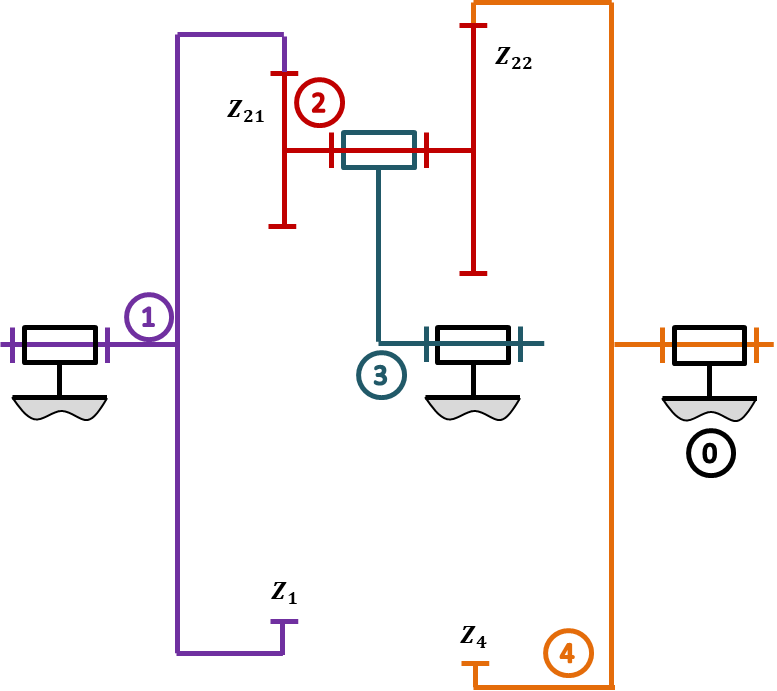
\includegraphics[width=.6\linewidth]{images/TrainEpi_03.png}
\end{center}



\subparagraph{}
\textit{Déterminer $\omega_{40}$ en fonction de  $\omega_{30}$ et $\omega_{10}$.}
\ifprof
 \begin{corrige}
 
 En bloquant le porte satellite, on a : $\dfrac{\omega_{43}}{\omega_{13}}=\dfrac{Z_{1}Z_{22}}{Z_{21}Z_{4}}$.
  On a donc, 
  $\dfrac{\omega_{40}+\omega_{03}}{\omega_{10}+\omega_{03}}=
\dfrac{Z_{1}Z_{22}}{Z_{21}Z_{4}}$

  $\Leftrightarrow \omega_{40}+\omega_{03}=\dfrac{Z_{1}Z_{22}}{Z_{21}Z_{4}}\left( \omega_{10}+\omega_{03} \right)$
 
 $\Leftrightarrow \omega_{40}=\dfrac{Z_{1}Z_{22}}{Z_{21}Z_{4}}\left( \omega_{10}-\omega_{30} \right) + \omega_{30}$

 $\Leftrightarrow \omega_{40}=\dfrac{Z_{1}Z_{22}}{Z_{21}Z_{4}}\omega_{10} +\left(1- \dfrac{Z_{1}Z_{22}}{Z_{21}Z_{4}}\right)\omega_{30}$

 \end{corrige}
 \else
 \fi
 
\subparagraph{}
\textit{On suppose que $\omega_{40}$ est bloqué. Exprimer le rapport $\dfrac{\omega_{30}}{\omega_{10}}$.}
\ifprof
 \begin{corrige}
 $\Leftrightarrow 0=\dfrac{Z_{1}Z_{22}}{Z_{21}Z_{4}}\omega_{10} +\left(1- \dfrac{Z_{1}Z_{22}}{Z_{21}Z_{4}}\right)\omega_{30}$

$\Leftrightarrow  \dfrac{Z_{1}Z_{22}}{Z_{21}Z_{4}}\omega_{10} =-\left(1- \dfrac{Z_{1}Z_{22}}{Z_{21}Z_{4}}\right)\omega_{30}$

$\Leftrightarrow  \dfrac{\omega_{30}}{\omega_{10}} = \dfrac{ \dfrac{Z_{1}Z_{22}}{Z_{21}Z_{4}}}{ \dfrac{Z_{1}Z_{22}}{Z_{21}Z_{4}}-1}= \dfrac{ {Z_{1}Z_{22}}}{ {Z_{1}Z_{22}}-Z_{21}Z_{4}}$
 \end{corrige}
 \else
 \fi



Soit le train épicycloïdal suivant. 

\begin{center}
 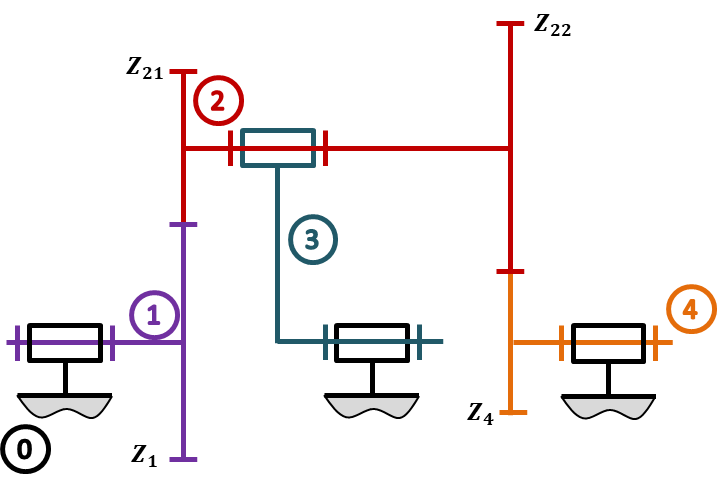
\includegraphics[width=.6\linewidth]{images/TrainEpi_04.png}
\end{center}



\subparagraph{}
\textit{Déterminer $\omega_{40}$ en fonction de  $\omega_{30}$ et $\omega_{10}$.}
\ifprof
 \begin{corrige}
 
 En bloquant le porte satellite, on a : $\dfrac{\omega_{43}}{\omega_{13}}=\dfrac{Z_{1}Z_{22}}{Z_{21}Z_{4}}$.
  On a donc, 
  $\dfrac{\omega_{40}+\omega_{03}}{\omega_{10}+\omega_{03}}=
\dfrac{Z_{1}Z_{22}}{Z_{21}Z_{4}}$

  $\Leftrightarrow \omega_{40}+\omega_{03}=\dfrac{Z_{1}Z_{22}}{Z_{21}Z_{4}}\left( \omega_{10}+\omega_{03} \right)$
 
 $\Leftrightarrow \omega_{40}=\dfrac{Z_{1}Z_{22}}{Z_{21}Z_{4}}\left( \omega_{10}-\omega_{30} \right) + \omega_{30}$

 $\Leftrightarrow \omega_{40}=\dfrac{Z_{1}Z_{22}}{Z_{21}Z_{4}}\omega_{10} +\left(1- \dfrac{Z_{1}Z_{22}}{Z_{21}Z_{4}}\right)\omega_{30}$

 \end{corrige}
 \else
 \fi
 
\subparagraph{}
\textit{On suppose que $\omega_{40}$ est bloqué. Exprimer le rapport $\dfrac{\omega_{30}}{\omega_{10}}$.}
\ifprof
 \begin{corrige}
 $\Leftrightarrow 0=\dfrac{Z_{1}Z_{22}}{Z_{21}Z_{4}}\omega_{10} +\left(1- \dfrac{Z_{1}Z_{22}}{Z_{21}Z_{4}}\right)\omega_{30}$

$\Leftrightarrow  \dfrac{Z_{1}Z_{22}}{Z_{21}Z_{4}}\omega_{10} =-\left(1- \dfrac{Z_{1}Z_{22}}{Z_{21}Z_{4}}\right)\omega_{30}$

$\Leftrightarrow  \dfrac{\omega_{30}}{\omega_{10}} = \dfrac{ \dfrac{Z_{1}Z_{22}}{Z_{21}Z_{4}}}{ \dfrac{Z_{1}Z_{22}}{Z_{21}Z_{4}}-1}= \dfrac{ {Z_{1}Z_{22}}}{ {Z_{1}Z_{22}}-Z_{21}Z_{4}}$
 \end{corrige}
 \else
 \fi


%
%\section*{Exercice 6 -- Train épicycloïdal -- Type 3}
%\setcounter{exo}{0}

\ifprof
\newpage
\else
\fi

\section*{Exercice 6 -- Train épicycloïdal -- Type 4 -- Poulie Redex}
\setcounter{exo}{0}

\textit{D'après ressources de Stéphane Genouël.}


\begin{obj}~\\
Vérifier les performances d'un réducteur.
\end{obj}

\ifprof
\else
Il existe 2 grandes familles de poulies Redex H ou SR, selon la forme de l’arbre central.


\begin{center}
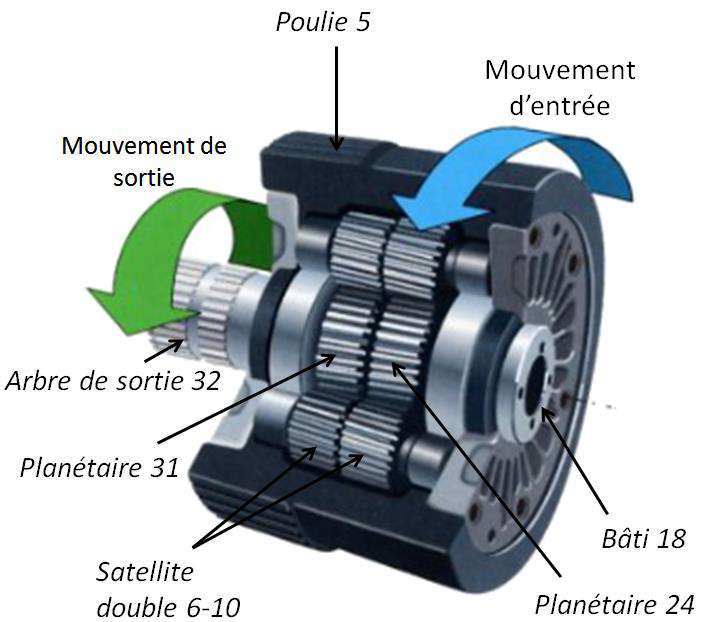
\includegraphics[width=.7\linewidth]{images/redex_01}
\end{center}



Le mouvement d’entrée est reçu par le boîtier tournant 5, entraîné par 5 courroies trapézoïdales 8, et guidé en rotation par rapport au bâti 18 à l’aide de deux roulements à billes 23 et 28. 
Les flasques 16 permettent le montage des organes intérieurs. Ils sont munis de joints d’étanchéité 22 et 29. 
Les trois axes 9, guidés en rotation par rapport au boîtier tournant 5 à l’aide de deux roulements à aiguilles 4 et 11, portent les trois satellites doubles 6-10.
Les liaisons encastrements entre les axes 9 et les satellites 6 et 10 sont assurées (élastiquement) par de la matière plastique injectée entre les axes et les pignons préalablement dentelés (voir coupe A-A et B-B). 
Les satellites 10 sont en prise avec le planétaire 24 (qui est en liaison encastrement avec le bâti 18 à l’aide d’un assemblage cannelé).
Les satellites 6 sont en prise avec le planétaire 31 (qui est en liaison encastrement avec l’arbre de sortie 32 à l’aide d’un assemblage cannelé). Cet arbre de sortie 32 est guidé en rotation par rapport au bâti 18 à l’aide de deux roulements à aiguilles 19 et 21.

\fi

\subparagraph{}
\textit{Déterminer littéralement, en fonction des nombres de dents, la loi E/S du système (c'est-à-dire le rapport de transmission).}

\ifprof
\begin{corrige}
On cherche $\dfrac{\omega_{30}}{\omega_{10}}$. En bloquant le porte satellite 1, on a  
$\dfrac{\omega_{31}}{\omega_{01}}=\dfrac{Z_0 Z_2 }{Z_2' Z_3}$. En décomposant les vitesses, on a :
$\dfrac{\omega_{30}-\omega_{10}}{\omega_{10}}=-\dfrac{Z_0 Z_2 }{Z_2' Z_3}$
$\Leftrightarrow \omega_{30}-\omega_{10}=-\dfrac{Z_0 Z_2 }{Z_2' Z_3}\omega_{10}$
$\Leftrightarrow \omega_{30}=\left(1-\dfrac{Z_0 Z_2 }{Z_2' Z_3}\right)\omega_{10}$
$\Leftrightarrow \dfrac{\omega_{30}}{\omega_{10}}=1-\dfrac{Z_0 Z_2 }{Z_2' Z_3}$.
AN : $ \dfrac{\omega_{30}}{\omega_{10}}=1-\dfrac{49 \times 34}{31 \times 46}=-0,17$
\end{corrige}
\else
\fi

%
%\begin{center}
%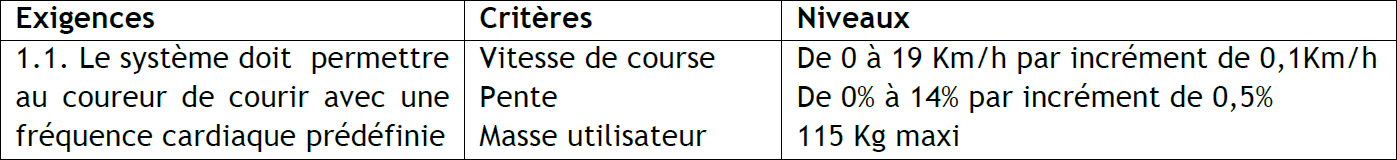
\includegraphics[width=.8\textwidth]{images/fig_02}
%\end{center}
%
%
\ifprof
\else
\begin{center}
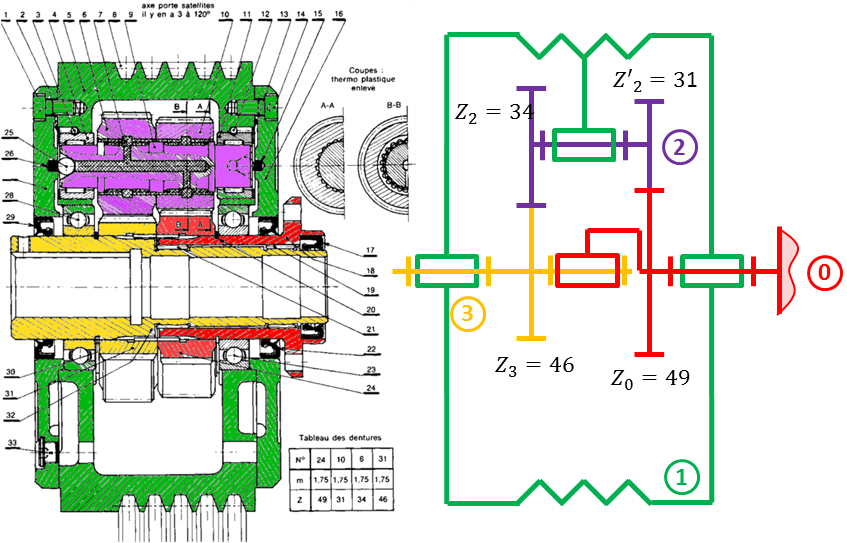
\includegraphics[width=\linewidth]{images/redex_04}
\end{center}
\fi



\section*{Exercice 7 -- {Broyeur à cisailles rotatives}}
\setcounter{exo}{0}
\textit{D'après BTS CPI -- 2015.}

\begin{obj}
Vérifier les performances d'un réducteur.
\end{obj}

\ifprof
\else

ECP Group est un fabricant européen spécialisé
dans la conception et la construction de machines
permettant la réduction du volume de ces D.I.B. au
moyen de broyeurs, de compacteurs ou de presses,
en favorisant la revalorisation, le recyclage ou le réemploi
de matières.

\begin{center}
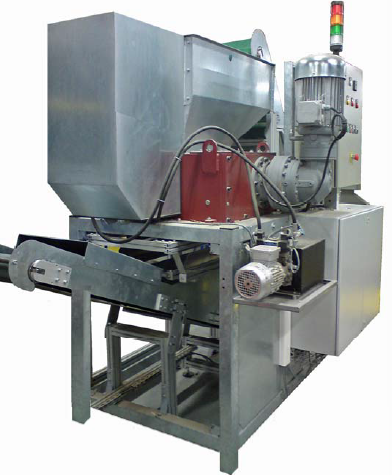
\includegraphics[width=.6\linewidth]{images/broyeur_01}
\end{center}

\begin{center}
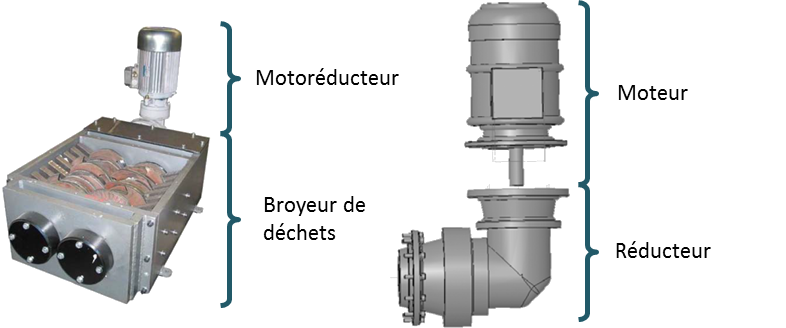
\includegraphics[width=\linewidth]{images/broyeur_04}
\end{center}

On donne un extrait du cahier des charges que doit respecter le broyeur.
\fi

\ifprof
\else
\begin{center}
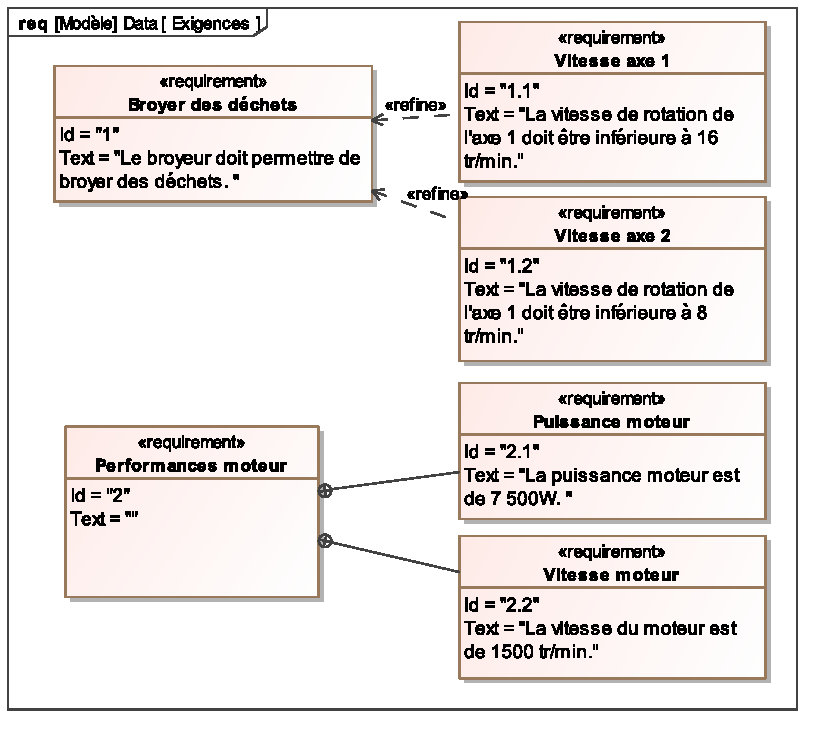
\includegraphics[width=\linewidth]{images/broyeur_06}
\end{center}

On donne le schéma cinématique du broyeur
\begin{center}
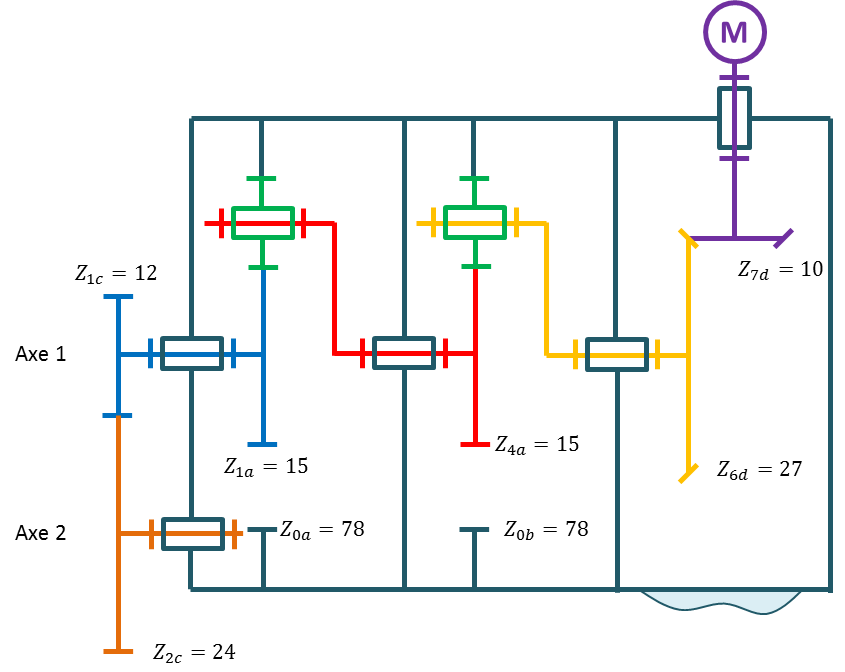
\includegraphics[width=\linewidth]{images/broyeur_05}
\end{center}

\fi

\subparagraph{}\textit{Donner les rapports de chacun des 4 étages de réduction.}
\ifprof
\begin{corrige}
\end{corrige}
\else
\fi

\subparagraph{}\textit{Vérifier que les exigences 1.1 et 1.2 sont satisfaites.}
\ifprof
\begin{corrige}
\end{corrige}
\else
\fi

\subparagraph{}\textit{Évaluer le couple de broyage sur chacun des axes.}
\ifprof
\begin{corrige}
\end{corrige}
\else
\fi



\section*{Exercice 8 -- Centrifugeuse des boues d'une station d'épuration.}
\setcounter{exo}{0}
\textit{D'après concours CCP -- MP 2012.}

\begin{obj} Déterminer la vitesse d'un moteur pour répondre au cahier des charges. 
\end{obj}
\ifprof
\else
\footnotesize{
\textit{Les boues sont constituées d’eau et de matière sèche. La siccité est le pourcentage massique de matière
sèche. Ainsi, une boue avec une siccité de 10\% présente une humidité de 90\%. Afin
d’incinérer les boues, il faut les déshydrater pour atteindre une siccité de 20\%. La déshydratation
mécanique par centrifugation permet de séparer l’eau des matières sèches dans les boues.
La centrifugation se base sur la différence de densité entre les matières sèches et l’eau présente dans
cette boue. La boue arrive avec une certaine vitesse horizontale par un coté de la centrifugeuse. L’eau 
traverse alors toute la centrifugeuse dans sa
zone centrale tandis que les matières en suspension sont plaquées contre le tambour extérieur du fait
de sa vitesse de rotation. Une vis intérieure, tournant dans le même sens que le tambour mais à une
vitesse plus importante, vient alors récupérer les boues et les évacuer en sens inverse de l’eau jusqu’à
la sortie latérale.}}


\normalsize

\begin{center}
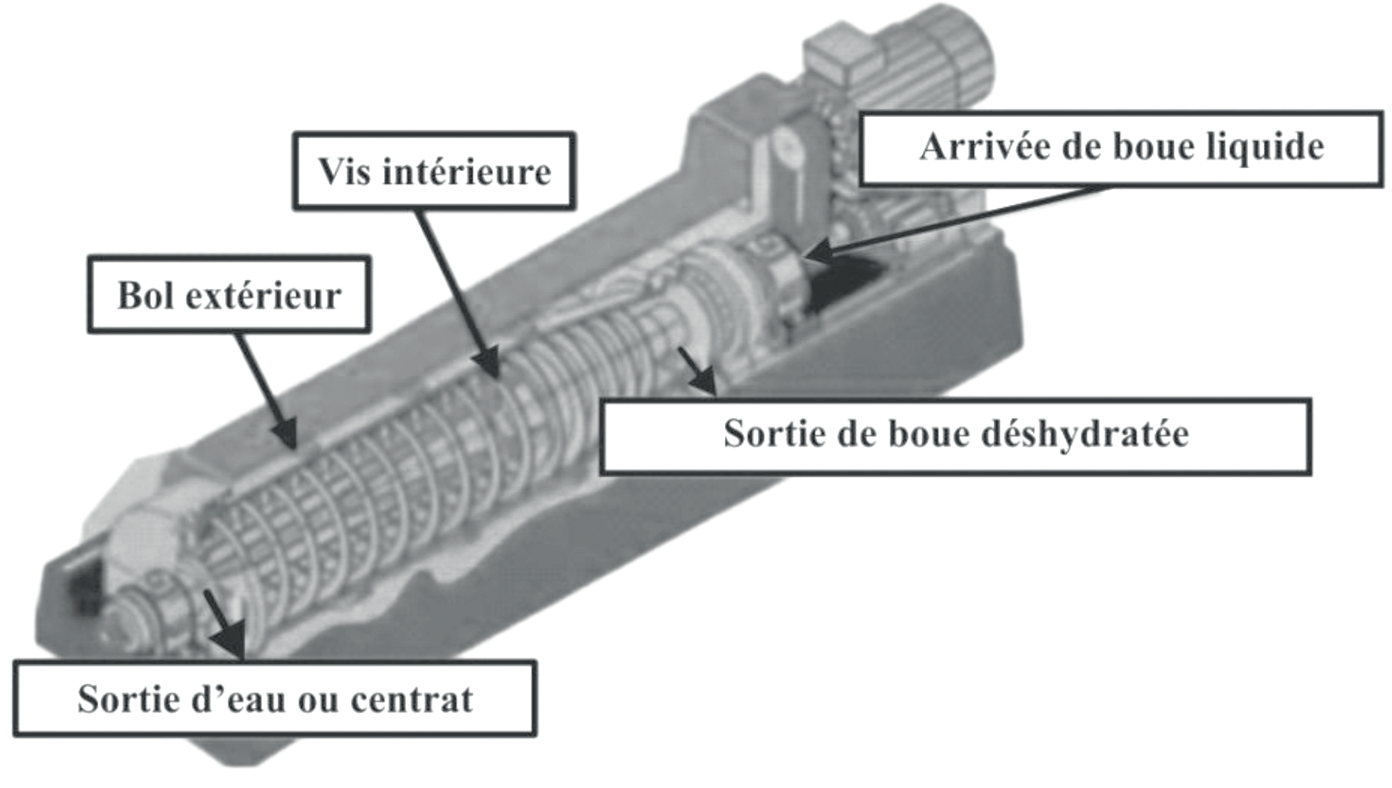
\includegraphics[width=\linewidth]{images/centrifugeuse_02}
\end{center}

La boue visqueuse est cisaillée par la différence de vitesse entre la vis et le tambour (bol extérieur).
La siccité de la boue est directement liée à cette différence de vitesse. On donne le diagramme des exigences partiel :

\begin{center}
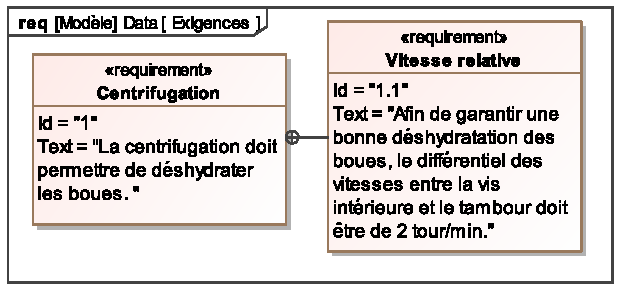
\includegraphics[width=.8\linewidth]{images/centrifugeuse_04}
\end{center}


La chaîne cinématique est représentée sur la figure
suivante.

\begin{center}
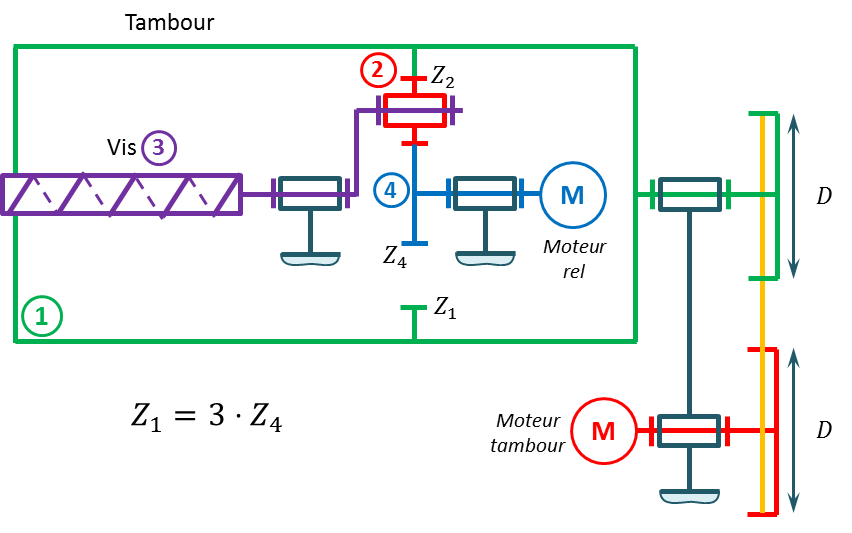
\includegraphics[width=\linewidth]{images/centrifugeuse_03}
\end{center}






La séquence de lancement de la centrifugeuse se déroule en trois phases :
\begin{itemize}
\item mise en marche du premier moteur $M_{\text{tambour}}$ jusqu’à ce que le tambour 1 atteigne sa vitesse
de consigne de 2 000 tours/min. Le moteur $M_{\text{rel}}$ est à l’arrêt;
\item mise en marche du deuxième moteur $M_{\text{rel}}$ jusqu’à ce que la vitesse différentielle de
2 tours/min soit atteinte entre le tambour 1 et la vis 3. La vis 3 tourne ainsi plus vite que le
tambour 1;
\item la boue liquide est ensuite introduite.
\end{itemize}

\fi


\subparagraph{}
\textit{Déterminer la fréquence de rotation de la vis (par rapport au bâti) lors de la phase de lancement.}
\ifprof
\begin{corrige}
\end{corrige}
\else
\fi

\subparagraph{}
\textit{Déterminer alors la fréquence de rotation que doit avoir le moteur <<rel>> pour respecter l'exigence 1.1.}
\ifprof
\begin{corrige}
\end{corrige}
\else
\fi



\section*{Exercice 9 -- Control'X -- Axe numérique asservi}
\setcounter{exo}{0}

\textit{ D'après documentation F. Mazet.} \\

\ifprof
\else
\begin{center}
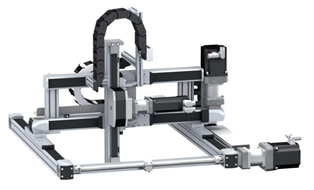
\includegraphics[width=\linewidth]{images/cx_01}
\end{center}

\begin{obj} Établir la loi entrée-sortie du transmetteur de mouvement. 
\end{obj}


On s'intéresse à la chaîne de transmission de puissance du Control'X dont un modèle est donné dans la figure ci-dessous.

On note : 
\begin{itemize}
\item \textbf{0:} le bâti auquel est encastré une couronne de rayon primitif $R_b$;
\item \textbf{1:} le pignon de sortie du moteur de rayon primitif $R_m$;
\item \textbf{2:} un des 3 satellites du réducteur épicycloïdal de rayon primitif $R_s$;
\item \textbf{3:} le porte-satellite auquel est encastré une poulie de rayon $R_p$;
\item \textbf{5:} le chariot de masse $M$ encastré à la courroie \textbf{4} considérée inextensible. On note $v=\vectv{D}{5}{0}\cdot \vect{y}$;
\item \textbf{3:} le seconde poulie de rayon $R_p$;
\end{itemize}
%La fréquence de rotation du moteur Man est de 1900 tr/min.


\fi

\subparagraph{}
\textit{Déterminer la relation entre $\omega(1/0)$ et $v$.}

\ifprof
\begin{corrige}

\end{corrige}
\else
\fi


\ifprof
\else 
\begin{center}
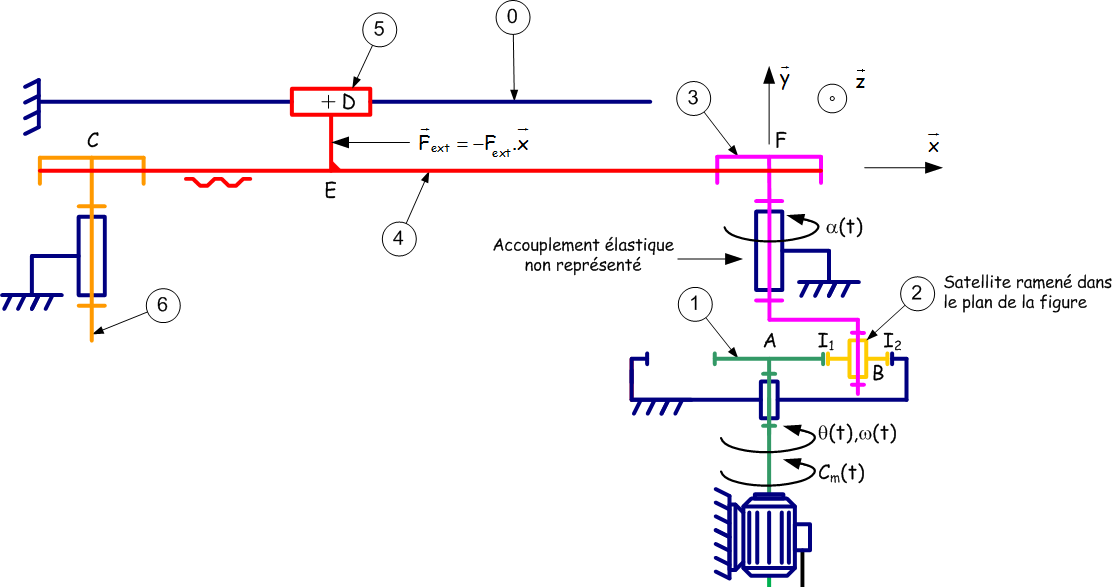
\includegraphics[width=\linewidth]{images/cx_02}
\end{center}
\fi

\section*{Exercice 10 -- Transmission à variation continue -- Vario Fendt}
\setcounter{exo}{0}

\textit{D'après concours CCP -- MP 2008.}

\begin{obj} 
Établir les relations cinématiques dans une transmission mécanique de tracteur.
\end{obj}

\ifprof
\else

On s'intéresse à la chaîne de transmission de puissance d'un tracteur Fendt. Cette dernière est composée d'un moteur (et d'une pompe) hydraulique (Mh) ainsi que d'un moteur thermique MAN (Mm). 

Le moteur MAN a pour but de fournir de la puissance à la pompe hydraulique et au tracteur (récepteur R). On donne ci-dessous le schéma de la transmission. 
 
\begin{center}
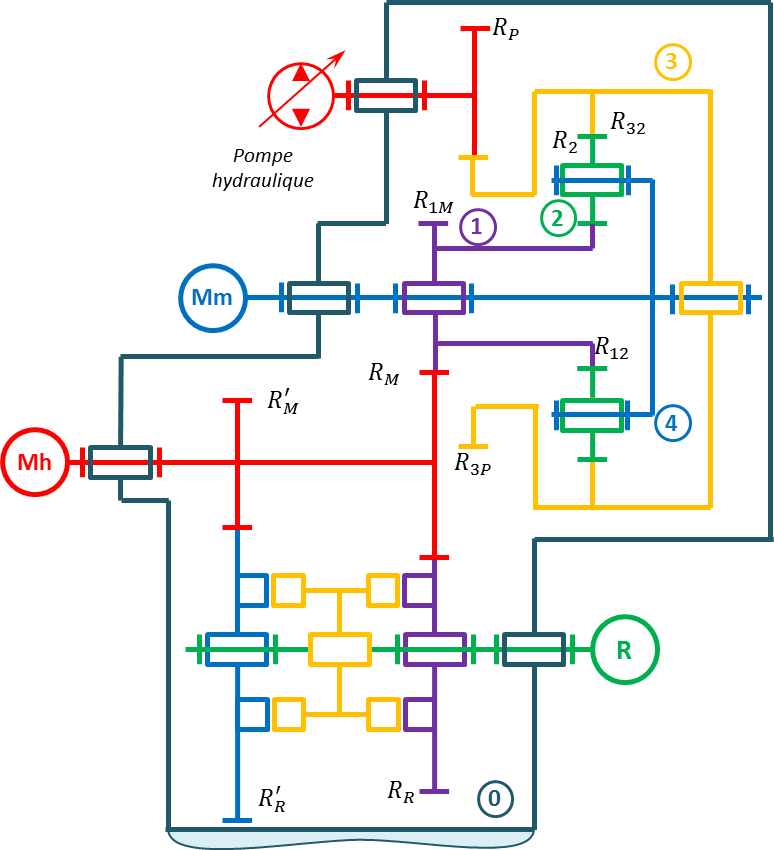
\includegraphics[width=\linewidth]{images/fendt_02}
\end{center}

Les rayons des pignons sont les suivants : $R_{12}=60$, $R_{1M}=33$, $R_{2}=30$, $R_{32}=120$, $R_{3P}=54$, $R_{M}=54$, $R'_{M}=48$, $R_{R}=42$, $R'_{R}=48$. 

Une étude antérieure a permis d'établir que $\dfrac{\omega(Ph/0)}{\omega(Mh/0)} = \dfrac{2y}{x}$ avec $x\in[0,71;1]$ et $y\in[0;1]$.
%\begin{center}
%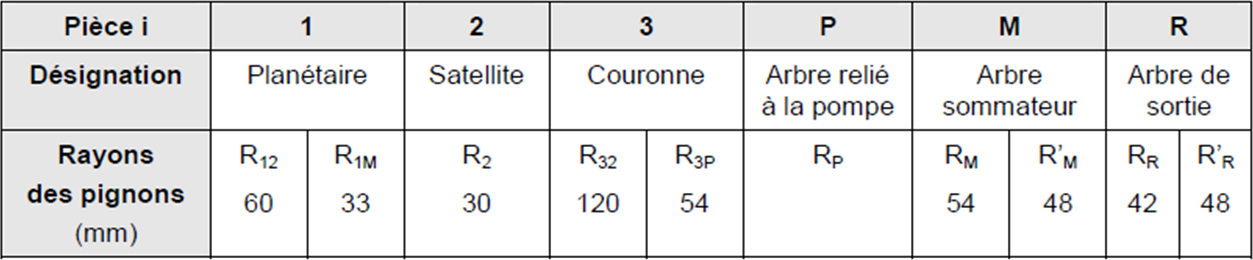
\includegraphics[width=\linewidth]{images/fendt_03}
%\end{center}

La fréquence de rotation du moteur Man est de 1900 tr/min.
\fi

\subparagraph{}
\textit{Déterminer la relation entre $\omega(1/0)$, $\omega(3/0)$ et $\omega(4/0)$}

\subparagraph{}
\textit{Montrer que la relation entre la rotation du moteur hydraulique et le moteur Man peut se mettre sous la forme : $\dfrac{\omega(Mh/0)}{\omega(Mm/0)}=-\dfrac{Ax}{BR_py + Cx}$ où on explicitera $A$, $B$ et $C$.}


\ifprof
\newpage
\begin{corrige}
On cherche une relation entre $\omega_{\text{Mh}/0}$, $\omega_{\text{Ph}/0}$ et $\omega_{\text{Mm}/0}$ (avec Mm et 4 même classe d'équivalence). Pour cela, on va d'abord rechercher une relation entre $\omega(3/0)$, $\omega(4/0)$ et $\omega(1/0)$.

Bloquons le porte satellite 4, directement lié au moteur Mm. On est alors en présence d'un réducteur simple d'entrée  $\omega(1/4)$ et de sortie $\omega(3/4)$. On a donc : 
$\dfrac{\omega(3/4)}{\omega(1/4)} = -\dfrac{R_{12}}{R_{32}}$. 

En libérant le porte satellite, on a donc :
$ \dfrac{\omega(3/4)}{\omega(1/4)}
= \dfrac{\omega(3/0)-\omega(4/0)}{\omega(1/0)-\omega(4/0)}
= -\dfrac{R_{12}}{R_{32}}
\Leftrightarrow 
R_{32} \omega(3/0) +R_{12}\omega(1/0) = \omega(4/0)\left(R_{12}+R_{32}\right)$

On a donc, $R_{32} \omega(3/0) +R_{12}\omega(1/0) = \omega(\text{Mm}/0)\left(R_{12}+R_{32}\right)$.

Par ailleurs, $\dfrac{\omega(\text{Ph}/0)}{\omega(3/0)} = -\dfrac{R_{3P}}{R_P}$ et 
$\dfrac{\omega(1/0)}{\omega(\text{Mh}/0)} = -\dfrac{R_M}{R_{1M}}$.

On a donc, $ \dfrac{2y}{x} \omega(Mh/0)= -\omega(3/0)\dfrac{R_{3P}}{R_P} \Leftrightarrow  \omega(3/0) = -\dfrac{2y}{x} \dfrac{R_P}{R_{3P}}\omega(Mh/0)$.

En utilisant la relation du train épi :
On a donc, $-R_{32} \dfrac{2y}{x} \dfrac{R_P}{R_{3P}}\omega(Mh/0)  -R_{12} \dfrac{R_M}{R_{1M}} \omega(\text{Mh}/0) = \omega(\text{Mm}/0)\left(R_{12}+R_{32}\right) \Leftrightarrow \left(-R_{32} \dfrac{2y}{x} \dfrac{R_P}{R_{3P}}  -R_{12} \dfrac{R_M}{R_{1M}} \right)\omega(\text{Mh}/0) = \omega(\text{Mm}/0)\left(R_{12}+R_{32}\right)$.


$\dfrac{\omega(Mh/0)}{\omega(Mm/0)}=-\dfrac{R_{12}+R_{32}}{R_{32} \dfrac{2y}{x} \dfrac{R_P}{R_{3P}}  +R_{12} \dfrac{R_M}{R_{1M}}}$

$\dfrac{\omega(Mh/0)}{\omega(Mm/0)}=-\dfrac{\left( R_{12}+R_{32}\right)R_{1M} R_{3P}x }{R_{32} 2y R_PR_{1M} + R_{3P}xR_{12} R_M}$. 
On a donc, $A=\left( R_{12}+R_{32}\right)R_{1M} R_{3P}$, $B=R_{32} 2R_{1M}$ et $C= R_{3P}xR_{12} R_M$. 
\textbf{Attention, plusieurs solutions possibles, si on factorise le numérateur et le dénominateur par l'un ou l'autre des rayons.}
\end{corrige}
\else
\fi
%
%\section*{Exercice 8 -- Poulies -- courroies}
%\setcounter{exo}{0}
%
%\section*{Exercice 9 -- Roulement sans glissement}
%\setcounter{exo}{0}

\section*{Exercice 11 -- Transmission vis -- écrou}
\textit{D'après ressources Pole Chateaubriand -- Joliot-Curie.}
\setcounter{exo}{0}

\ifprof
\else

La conduite en ville nécessite des répétitions
fréquentes de la manœuvre d’embrayage /
débrayage. Pour améliorer le confort de conduite,
on peut substituer la force musculaire du
conducteur par une commande électrique de
l’embrayage. Dans ce cas, il devient nécessaire de
renseigner l’unité de contrôle électronique sur les
intentions du conducteur à partir d’un capteur de
position placé sur la pédale d’embrayage.
L’automatisation de la fonction embrayage
permet de corriger les éventuelles fausses
manœuvres du conducteur, d’assurer la fonction
anti-calage du moteur et de participer aux
fonctions d’anti-patinage et d’anti-blocage des
roues.

\begin{center}
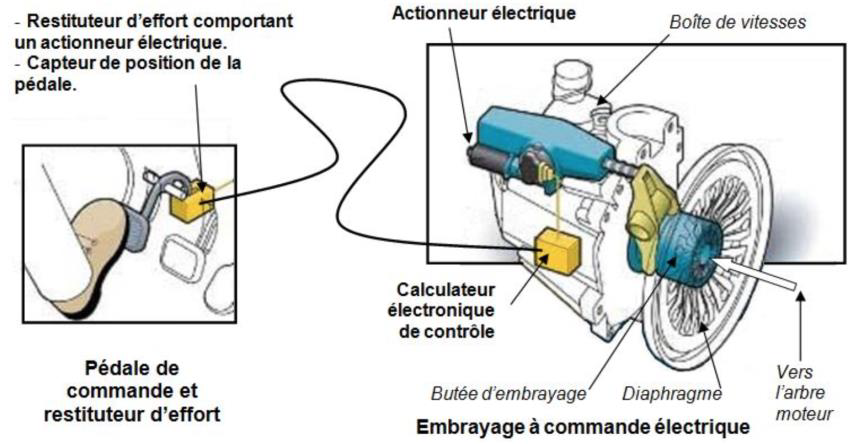
\includegraphics[width=\linewidth]{images/rest_01}
\end{center}


En cas d’utilisation de la pédale, il faut recréer les sensations
au conducteur, c'est-à-dire une résistance mécanique proche
de celle d’une commande mécanique classique. Pour réaliser
ce système de retour d’effort la solution peut être passive (un
ressort, par exemple) ou utiliser un système actif (à l’aide d’un
actionneur électrique), objet de l’étude.
L’étude porte sur un démonstrateur de restituteur actif
d’effort à la pédale. Le démonstrateur permet de tester
différentes lois de restitution d’effort pour rechercher la plus
ergonomique. Le système contrôle, par l’intermédiaire d’un
piston, l’effort sur la tige de poussée de la pédale.


\begin{center}
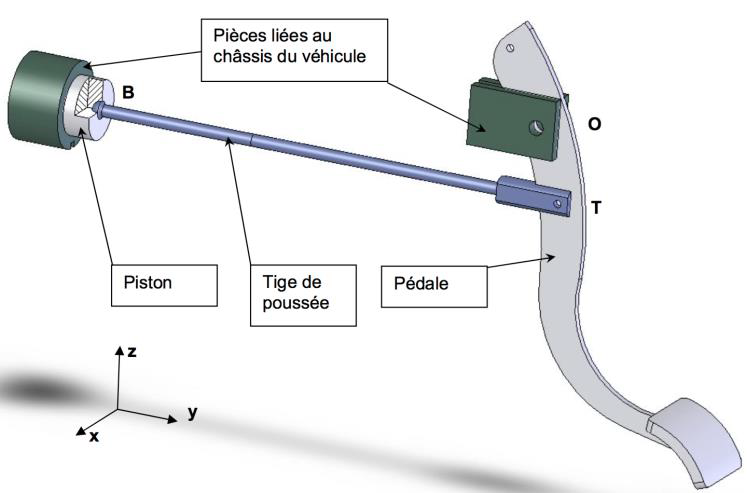
\includegraphics[width=\linewidth]{images/rest_02}
\end{center}

Le schéma du restituteur actif est donné ci-dessous. Le pas de la vis est $p_v =\SI{10}{mm}$.
Le diamètre de la poulie 2 est le double de celui de la poulie 1. 


\begin{center}
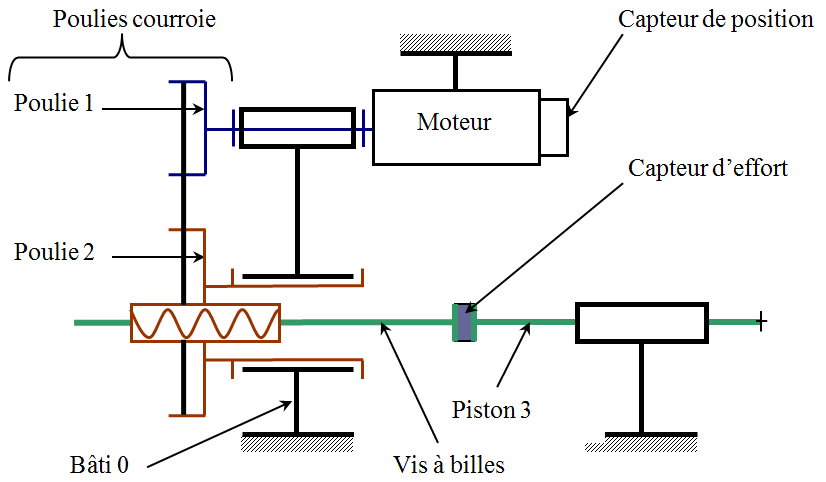
\includegraphics[width=\linewidth]{images/rest_03}
\end{center}
\fi
\begin{obj}
Déterminer la première partie
de la loi entrée/sortie en vitesse du
système.
\end{obj}

\subparagraph{}
\textit{Sur le schéma cinématique, repasser chaque solide d’une couleur différente.}

\ifprof
\begin{corrige}
\end{corrige}
\else
\fi

\subparagraph{}
\textit{Compléter la chaîne d’énergie-puissance partielle en définissant les noms des transmetteurs et les grandeurs
d’entrée et de sortie cinématiques.}

\ifprof
\begin{corrige}
\end{corrige}
\else
\fi



\begin{center}
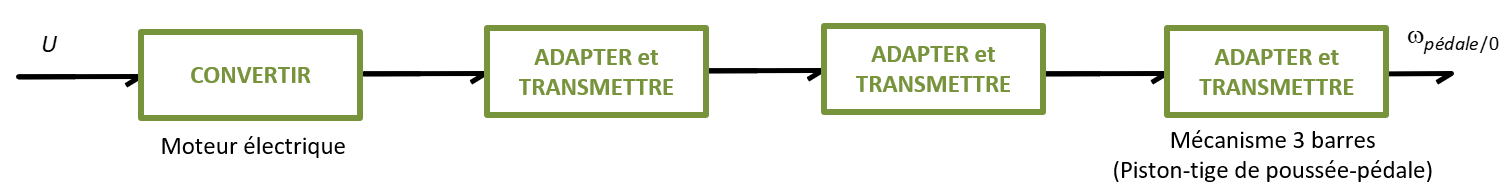
\includegraphics[width=\linewidth]{images/rest_04}
\end{center}

\subparagraph{}
\textit{Définir la loi entrée-sortie entre la vitesse de translation du piston 3 et la vitesse de rotation du moteur~1. }

\ifprof
\begin{corrige}
\end{corrige}
\else
\fi


\section*{Exercice 12 -- Axe de machine-outil à commande numérique}
\textit{D'après ressources Pole Chateaubriand -- Joliot-Curie.}
\setcounter{exo}{0}

\ifprof
\else
L’usinage est une opération de transformation d’un produit par enlèvement de matière.
Cette opération est à la base de la fabrication de produits dans les industries mécaniques.
La génération d’une surface par enlèvement de matière est obtenue grâce à un outil muni
d’au moins une arête coupante. Les différentes formes de pièces sont obtenues par des
translations et des rotations de l'outil par rapport à la pièce.

\begin{center}
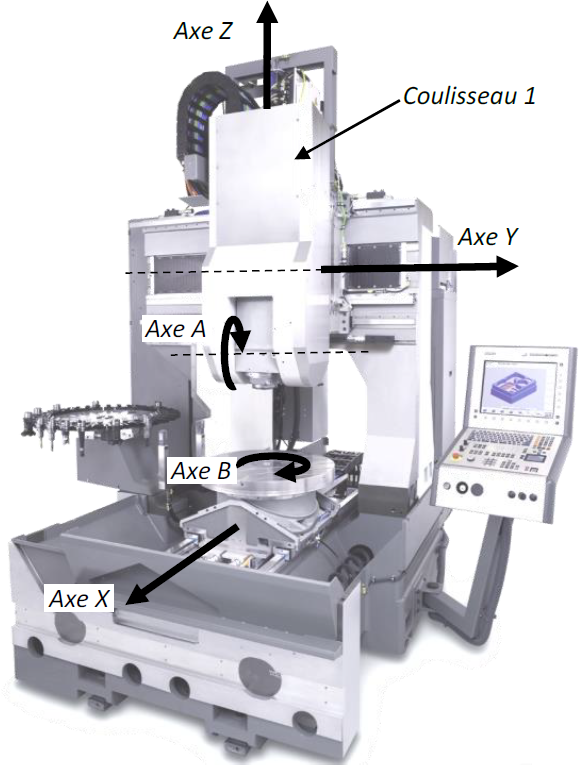
\includegraphics[width=.6\linewidth]{images/ugv_01}
\end{center}

On s’intéresse ici à l’axe Y qui met en mouvement le coulisseau 1,
sur lequel est fixée l’outil, par rapport au bâti 0. Le coulisseau 1 est mis en mouvement par un moteur
électrique qui délivre un couple moteur $C_m(t)$.

\begin{center}
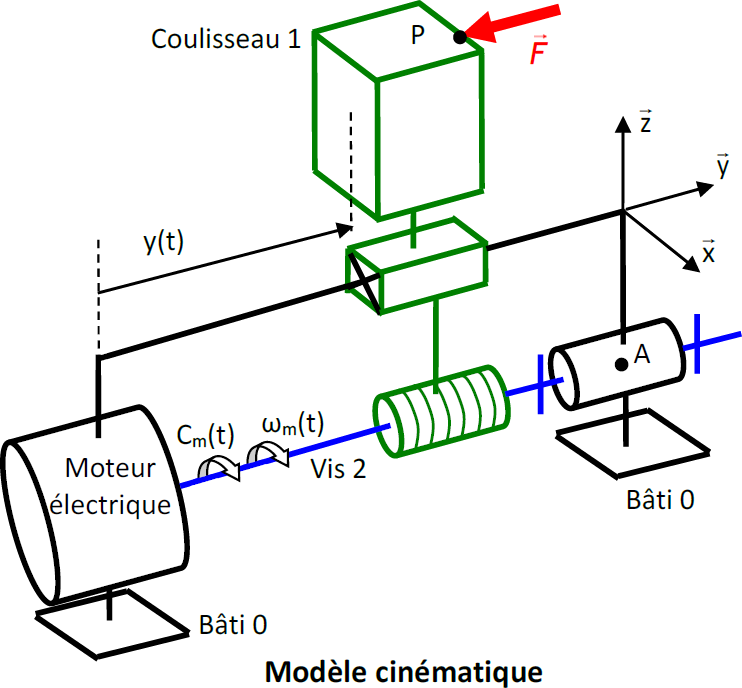
\includegraphics[width=\linewidth]{images/ugv_02}
\end{center}

On note $p$ le pas de vis. 
\fi


\subparagraph{}
\textit{Définir la loi entrée-sortie entre la vitesse de translation du coulisseau et la vitesse de rotation du moteur. }
\ifprof
\begin{corrige}
\end{corrige}
\else
\fi


\section*{Exercice 13 -- Treuil de levage}
\textit{D'après ressources Pole Chateaubriand -- Joliot-Curie.}
\setcounter{exo}{0}
\ifprof
\else
On s’intéresse à un treuil dont la photo et le modèle cinématique sont donnés ci-dessous.
\begin{center}
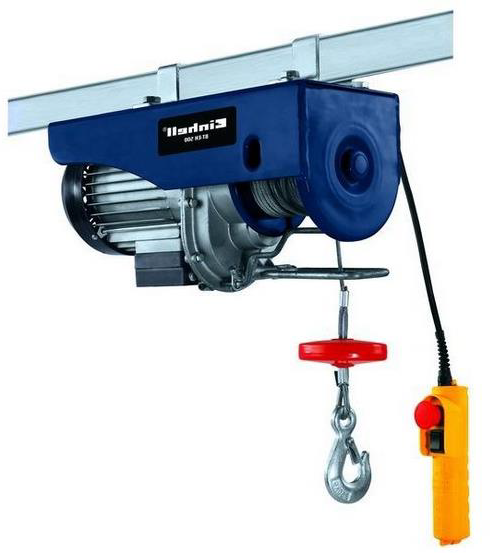
\includegraphics[width=.5\linewidth]{images/treuil_01}
\end{center}

\begin{center}
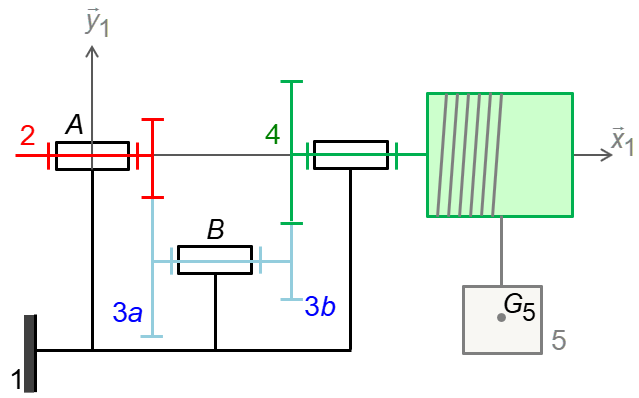
\includegraphics[width=\linewidth]{images/treuil_02}
\end{center}

On note $Z_2$ le nombre de dents de la roue dentée de l'arbre 2. On note l'arbre intermédiaire 3 et $Z_{3a}$ et $Z_{3b}$ les nombres de dents de ses deux roues dentées. On note $R$ le rayon du tambour 4 sur lequel s’enroule sans glisser un câble et $Z_4$ le nombre de dents de sa roue dentée.

\fi

\subparagraph{}
\textit{Déterminer la relation entre $v_{51}$ la vitesse de déplacement de la charge par rapport au bâti et $\omega_{21}$ la vitesse de rotation du moteur.}
\ifprof
\begin{corrige}
\end{corrige}
\else
\fi


\subparagraph{}
\textit{On note $J_2$, $J_3$, $J_4$ l'inertie des pièces 2, 3 et 5. On note $M_5$ la masse du solide 5. Donner la masse équivalente ramenée << à la translation >> de la masse. Donner l'inertie équivalente ramenée à l'arbre d'entrée 2.  }
\ifprof
\begin{corrige}
\end{corrige}
\else
\fi


\ifprof
\end{multicols}
\else
\end{multicols}
\fi

\end{document}

\subparagraph{}
\textit{}

\ifprof
\begin{corrige}
\end{corrige}
\else
\fi

	